\documentclass[handout,usepdftitle=false,xcolor=dvipsnames,aspectratio=169]{beamer}
%\documentclass[beamer,usepdftitle=false,xcolor=dvipsnames,aspectratio=169]{beamer}
%\documentclass[trans,notes=show,usepdftitle=false,aspectratio=169]{beamer}


\usepackage[english]{babel}
\usepackage{iftex}
\ifPDFTeX
\usepackage[T1]{fontenc}
\usepackage[utf8]{inputenc}
\usepackage{lmodern}
\else
\usepackage{fontspec}
\defaultfontfeatures{Ligatures=TeX}
\setmainfont{Latin Modern Roman}
\setsansfont{Latin Modern Sans}
\setmonofont{Latin Modern Mono}
\usepackage{newunicodechar}
\newfontfamily\unicodeSymbolFont{Segoe UI Symbol}[
  BoldFont=Segoe UI Symbol,
  ItalicFont=Segoe UI Symbol,
  BoldItalicFont=Segoe UI Symbol
]
\newunicodechar{⟂}{{\unicodeSymbolFont ⟂}}
\fi
\usepackage{amsmath,amsfonts}
\usepackage{booktabs,multirow,xcolor,colortbl}
\usepackage{bm}%to use a more powerful version of \boldsymbol
\usepackage{fvextra}
\usepackage{csquotes}
\usepackage{textcomp}
\ifPDFTeX
\DeclareUnicodeCharacter{27C2}{\ensuremath{\perp}}
\fi

\newcommand{\AllSample}{ \mathcal Y^T }

\usepackage[citestyle=authoryear-comp,bibstyle=../Preamble/mystyle_lowercase,maxbibnames=5,minbibnames=1,maxnames=2, minnames=1,datezeros=false,date=long,isbn=false,url=false,backend=biber,useprefix=true]{biblatex}
\addglobalbib{../Preamble/Macro_database_biblatex.bib}	

\usepackage{upquote}
\usepackage{ragged2e}
\usepackage{microtype}

\usepackage{multimedia}
\usepackage{graphicx}
\usepackage[export]{adjustbox}
\usepackage{epstopdf}
\usepackage[labelfont=bf,format=hang, figurename=Fig.]{caption}
\usepackage[subrefformat=parens,labelformat=empty]{subcaption}
\usepackage{pgfpages} % for multiple-screen presentations

\usepackage{array}

\newcolumntype{L}[1]{>{\RaggedRight\let\newline\\\arraybackslash\hspace{0pt}}m{#1}}
\newcolumntype{C}[1]{>{\centering\let\newline\\\arraybackslash\hspace{0pt}}m{#1}}
\newcolumntype{R}[1]{>{\raggedleft\let\newline\\\arraybackslash\hspace{0pt}}m{#1}}
%https://tex.stackexchange.com/questions/12703/how-to-create-fixed-width-table-columns-with-text-raggedright-centered-raggedlef


%%% use serif font for math
\usefonttheme[onlymath]{serif}

%%% define blue highlighting
\newcommand{\highlight}[1]{{\color{blue}{#1}}}

%%%% define command for setting sources

\newcommand{\Source}{}

%%%
\beamertemplatenavigationsymbolsempty


%%% define themes
\usetheme{Boadilla}
\usecolortheme{rose}
\usecolortheme[named=blue]{structure}

\newcommand\textbox[1]{%
  \parbox{.333\textwidth}{#1}%
}

\setbeamertemplate{sections/subsections in toc}[sections numbered]


%%%% set coloring in  foot and head
\setbeamercolor{alerted text}{fg=red!80!black}
\setbeamertemplate{enumerate items}[default] % numbers enumerate items without encircling them
\setbeamertemplate{itemize items}[ball] % numbers enumerate items without encircling them
\setbeamercolor{section in head/foot}{fg=black, bg=white}
\setbeamercolor{subsection in head/foot}{fg=black, bg=white}
\setbeamercolor{title}{fg=black}
\setbeamercolor{subtitle}{fg=blue}

\setbeamertemplate{caption}[numbered]

%%% set overlays as default
\beamerdefaultoverlayspecification{<+->}

%%%% settings for output mode

\mode<beamer>
{
%\setbeameroption{show notes on second screen=right}
}

\mode<trans>
{\renewcommand{\highlight}[1]{{\textbf{#1}}}}


\mode<handout>
{
\renewcommand{\highlight}[1]{{\textbf{#1}}}
%\pgfpagesuselayout{4 on 1}[a4paper,border shrink = 5mm,landscape]
%\setbeamercolor{background canvas}{bg=black!5}
}


%%% define Exercise counter
\newcounter{Exercise}
\resetcounteronoverlays{Exercise}
\setcounter{Exercise}{0}
\newcommand{\Exercise}{\refstepcounter{Exercise}\emph{\structure{Übung \theExercise}: }}

%%%% define environments for theorems etc and make them numbered
\setbeamertemplate{theorems}[numbered]

\newtheorem{assum}{Assumption}
\setbeamertemplate{assum}[numbered]

\newtheorem{defin}{Definition}
\setbeamertemplate{defin}[numbered]

\newtheorem{propos}{Proposition}
\setbeamertemplate{propos}[numbered]


%%%% Make Parts show up in TOC
\makeatletter
\AtBeginPart{%
  \addtocontents{toc}{\protect\beamer@partintoc{\the\c@part}{\beamer@partnameshort}{\the\c@page}}%
}
%% number, shortname, page.
\providecommand\beamer@partintoc[3]{%
  \ifnum\c@tocdepth=-1\relax
    % requesting onlyparts.
    \makebox[6em]{#1.} #2
    \par
  \fi
}
\define@key{beamertoc}{onlyparts}[]{%
  \c@tocdepth=-1\relax
}
\makeatother%

%%%% fix bug in beamer package with note itemize
%%% http://tex.stackexchange.com/questions/1480/changing-the-textwidth-of-the-notes-in-beamer-repost-from-so
\makeatletter
\defbeamertemplate{note page}{infolines}
{%
  \vskip.75em
  \nointerlineskip
  \begin{minipage}{\textwidth} % this is an addition
  \footnotesize \insertnote
  \end{minipage}               % this is an addition
}
\makeatother

\setbeamertemplate{note page}[infolines]


\newcommand{\backupbegin}{
   \newcounter{framenumberappendix}
   \setcounter{framenumberappendix}{\value{framenumber}}
}
\newcommand{\backupend}{
   \addtocounter{framenumberappendix}{-\value{framenumber}}
   \addtocounter{framenumber}{\value{framenumberappendix}}
}

\hypersetup{bookmarksnumbered=true,naturalnames=true,pdfhighlight=/N,citebordercolor={1 1
1},linkbordercolor={1 1 1},colorlinks=true,anchorcolor=black,linkcolor=blue,citecolor=green,urlcolor=green,
pdfpagemode=UseOutlines,breaklinks=true,
pdfkeywords=Dynare, pdfsubject=Dynare,pdfstartpage=1} %pdfpagemode=fullpage

\usepackage[copyright]{ccicons}

\usepackage{tikz,pgfplots}
\pgfplotsset{compat=1.18}
\usetikzlibrary{arrows,calc,decorations.pathreplacing,decorations.shapes}
\pgfdeclarelayer{background}
\pgfdeclarelayer{foreground}
\pgfsetlayers{background,main,foreground}

\usepackage{relsize}
\newcommand\LM{\ensuremath{\mathit{LM}}}
\newcommand\IS{\ensuremath{\mathit{IS}}}
\DeclareMathOperator{\std}{std}


\setbeamertemplate{footline}{
\begin{beamercolorbox}{subsection in head/foot}
\insertsectionnavigationhorizontal{.95\textwidth}{\hskip0pt
\hfill}{\hfill \insertframenumber /\inserttotalframenumber}
\end{beamercolorbox}
}

\newenvironment{witemize}{\itemize\addtolength{\itemsep}{8pt}}{\enditemize}
\newenvironment{wenumerate}{\enumerate\addtolength{\itemsep}{8pt}}{\endenumerate}

\usepackage[]{minted}
\usepackage{tcolorbox}
\usepackage{etoolbox}
\BeforeBeginEnvironment{minted}{\begin{tcolorbox}[boxsep=0mm]}%
\AfterEndEnvironment{minted}{\end{tcolorbox}}%

\AtBeginEnvironment{minted}{%
  \renewcommand{\fcolorbox}[4][]{#4}}  

\newenvironment{wideitemize}{\itemize\addtolength{\itemsep}{10pt}}{\enditemize}
\newenvironment{wideenumerate}{\enumerate\addtolength{\itemsep}{10pt}}{\endenumerate}
\newcommand{\hi}[1]{{\color{beamer@blendedblue}#1}}


\title[]{\textbf{Advanced Dynare\\}
\medskip{Chapter XIII}\\
\emph{Solving Models with Occasionally Binding Constraints}
}

\author{Johannes Pfeifer}
\input{../date_place.txt}

\AtBeginSection[]
{
  \begin{frame}
    \frametitle{Outline}
    \tableofcontents[currentsection]
  \end{frame}
}


\begin{document}

\begin{frame}
  \titlepage
\end{frame}

% LTeX: language=en-US

\section{Introduction}
\begin{frame}{Overview}
	\begin{wideitemize}
        \item Focus on models with \hi{occasionally binding constraints}
        \item Since Dynare 5: implementation of OccBin toolkit to solve models with occasionally binding constraints
        \item Feature only recently added\\
        $\rightarrow$ please report any bugs you may encounter
    \end{wideitemize}
\end{frame}

\begin{frame}{Occasionally binding constraints}
	\begin{wideitemize}
        \item Historically, economists relied on linearized models:
            \begin{wideitemize}
                \item Useful to gain intuition
                \item Easy to apply, especially for estimation (linear state space tools)
            \end{wideitemize}
        \item However: many interesting economic problems and policy questions feature nonlinearities such as \hi{occasionally binding constraints (OBCs)}:
        \begin{wideitemize}
            \item effective lower bound on nominal interest rates \parencite{ChristianoEichenbaumRebelo2011}
            \item Credit constraints \parencite{GuerrieriIacoviello2017}
            \item Downward nominal wage rigidities \parencite{SGU2016}
        \end{wideitemize}
        \item Not always sensible to assume OBC is always binding as in e.g.\ \textcite{Iacoviello2005} or \textcite{JermannQuadrini2012}
    \end{wideitemize}
\end{frame}


\begin{frame}{Occasionally Binding Constraints in Dynare}
	\begin{wideitemize}
        \item Dynare essentially offers three options to solve models with occasionally binding constraints:
        \begin{wideenumerate}
	    \item Nonlinear perfect foresight models: brute force (\texttt{max/min}-operators) and mixed complementarity problems (MCP)
	    \item Linearized stochastic models with surprise shocks: OccBin
        \item Stochastic nonlinear models: Extended Path
        \end{wideenumerate}
	    %\item Model estimations via Bayesian techniques or maximum likelihood, including models with OBCs
	\end{wideitemize}
\end{frame}


\begin{frame}{Crucial distinction: informational structure}

\begin{enumerate}
 \item deterministic/perfect foresight: all future shocks are known exactly
  \item stochastic simulations: only the shock distributions are known
\end{enumerate}

\begin{columns}[T]
\column{0.5\linewidth}
\begin{wideitemize}
    \item \hi{Deterministic:}
     \begin{itemize}
	        \item[+] Arbitrary precision
	        \item[+] Easily captures nonlinearities (such as OBCs)
	        \item[--] Assumption of perfect foresight
	        \item[--] How to simulate time series?
	    \end{itemize}
\end{wideitemize}
\column{0.5\linewidth}
\begin{wideitemize}
    \item \hi{Stochastic:}
	      \begin{itemize}
	        \item[+] Captures uncertainty
	        \item[+] Needed for estimation with state space form
            \item[--] Typically suffers from curse of dimensionality
	        \item[+] Perturbation methods can capture OBCs with additional tools (OccBin)
	        \item[--] Often uses 1st order approximations: certainty equivalence
	    \end{itemize}
\end{wideitemize}
\end{columns}
\end{frame}


\begin{frame}{Outline}
  \tableofcontents
\end{frame}

\section[Prototype model]{A prototype model}
 \input{chapters/ProtoNKM.tex}

%\section[Dynare 101]{A fast-speed intro to Dynare}
%\begin{frame}{What is Dynare?}
%	\begin{wideitemize}
%	    \item A free software platform for handling a wide class of economic models, in particular, DSGE models: Dynare is a collection of Matlab routines.
%	    \item Dynare is very user-friendly and has low entry costs
%	    \item Users provide a \texttt{.mod} file containing parameters, model equations linking the variables, and a list of computing tasks to be performed.
%	    \item Provides many state-of-the-art algorithms to handle DSGE models
%	    \item \url{https://www.dynare.org/} See also the Dynare manual\footcite{adjemian2022dynare}, the forum \url{https://forum.dynare.org/} and other resources e.g. \href{https://drive.google.com/file/d/1DO1OK5AKLWfcJX49ZPCGo58Ni2LdERw4/view}{An Introduction to Graphs in Dynare}
%	\end{wideitemize}
%\end{frame}
%
%\begin{frame}{Tools available in Dynare}
%	\begin{wideitemize}
%	    \item Compute solutions to an approximation of stochastic models, including models with OBCs
%	    \item Compute solutions to deterministic models, including models with OBCs
%	    \item Model estimations via Bayesian techniques or maximum likelihood, including models with OBCs
%	    \item Solve for optimal policy...
%	    \item ...and many more
%	\end{wideitemize}
%\end{frame}
%
%\begin{frame}{How Dynare works}
%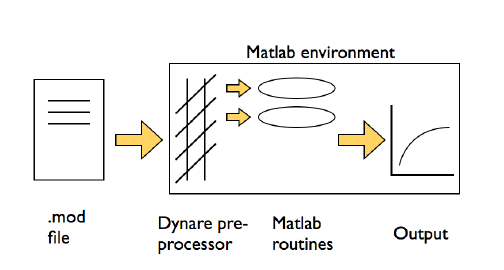
\includegraphics[width=0.8\textwidth]{figures/Dynare.PNG}\\
%\footnotesize{Source: Griffoli}
%\end{frame}


%\begin{frame}{A Dynare file}
%Our model:
%\begin{itemize}
%    \item Endogenous variables: $\pi_t, y_t, i_t, \varepsilon_t^a, \varepsilon_t^c, \varepsilon_t^i $
%    \item Some parameters: $ \beta, \kappa, \sigma,\phi_\pi,\phi_y,\rho^a, \rho^c, \rho^i $
%    \item Exogenous variables (shocks): $,u_t^a,u_t^c,u_t^i$ (see in the next slides)
%    \item Model equations
%    \begin{align*}
%        \pi_t =& \beta E_t\left[\pi_{t+1}\right]+\kappa y_t +\varepsilon_t^a \\
%        y_t =& E_t \left[y_{t+1} \right]- \frac{1}{\sigma}\left(i_t-E_t\left[\pi_{t+1}\right]\right)+\varepsilon_t^c \\
%        i_t =& \phi_\pi \pi_t + \phi_y y_t+\varepsilon_t^i
%        ...
%    \end{align*}
%\end{itemize}
%\end{frame}

%\begin{frame}{Structure of a Dynare file}
%\smartdiagramset{back arrow disabled,module minimum width=2.cm,font=\footnotesize}
%\smartdiagram[flow diagram:horizontal]{Preamble, Model definition, Steady state, Simulation and estimation}
%\begin{wideenumerate}
%\item Preamble: Declaration of endogenous and exogenous variables and parameters. Set value for calibrated parameters
%\item Model definition: State the dynamic model equations
%\item Steady state (long-run equilibrium)
%\item Additional computations: model checks,  simulation, estimation, ...
%\end{wideenumerate}
%\end{frame}

%\begin{frame}[fragile]{How to interact with Dynare: 1) Preamble}
%\begin{columns}
%\begin{column}[T]{0.5\textwidth}
%	    Our model:
%	    \begin{wideitemize}
%	        \item Endogenous variables: $\pi_t, y_t, i_t, \varepsilon_t^a, \varepsilon_t^c, \varepsilon_t^i$
%	        \item Exogenous variables (shocks): $u_t^a, u_t^c, u_t^i$
%	        \item Parameters: $ \beta, \kappa, \sigma,\phi_\pi,\phi_y,\rho^a,\rho^c,\rho^i $
%	    \end{wideitemize}
%\end{column}
%\begin{column}[T]{0.5\textwidth}
%Dynare code
%\begin{minted}{c++}
%var // endo vars
%pie y inom zeps_a zeps_c zeps_i;
%
%varexo
%u_a u_c u_i;
%
%parameters
%betta kappa sig phi_pi
%phi_y rho_a rho_c rho_i;
%\end{minted}
%\end{column}
%\end{columns}
%\end{frame}
%
%\begin{frame}[fragile]{How to interact with Dynare: 1) Preamble (cont'd)}
%\begin{columns}
%\begin{column}[T]{0.5\textwidth}
%	    \begin{wideitemize}
%	        \item Set $\beta$ and $\kappa$ to conventional values informed by real interest rates and price adjustment frequencies
%	        \item Choose parameters for the Taylor rule
%	        \item Set autocorrelation coefficients
%	        \item Unit intertemporal elasticity of substitution
%	    \end{wideitemize}
%\end{column}
%\begin{column}[T]{0.5\textwidth}
%\begin{minted}{c++}
%// Calibration
%betta   = 0.99;
%phi_pi  = 1.5;
%phi_y   = 0.2;
%kappa   = 0.12;
%rho_a   = 0.8;
%rho_c   = 0.8;
%rho_i   = 0.5;
%sig     = 1;
%\end{minted}
%\end{column}
%\end{columns}
%\end{frame}
%
\begin{frame}[fragile]{Dynare code: Core part of the model}
%\begin{columns}
%\begin{column}[T]{0.5\textwidth}
%	    \begin{wideitemize}
%	        \item Dynare allows writing the model in a very natural way
%	        \item Keyword \texttt{model;} indicates begin of model declaration. The argument \texttt{linear} instructs Dynare that our model is already linearised (the software can do it for you too)
%	        \item \texttt{(+1)} indicates expected (one-period ahead) variables. No expectations operator needed.
%	        \item \texttt{(-1)} indicates lagged variables
%	    \end{wideitemize}
%\end{column}
%\begin{column}[T]{0.5\textwidth}
\begin{minted}{c++}
model(linear);
[name='Phillips Curve']
pie=betta*pie(+1)+kappa*y+zeps_a;

[name='IS curve']
y=y(+1)-1/sig*(inom-pie(+1))+zeps_c;

[name='Notional rate Taylor rule']
inomnot=rhoinom*inomnot(-1)
        +(1-rhoinom)*(phi_pi*pie+phi_y*y)+zeps_i;
\end{minted}
%\end{column}
%\end{columns}
\end{frame}


%\begin{frame}[fragile]{Timing conventions}
%\begin{wideitemize}
%    \item A variable decided at time $t$ enters as a contemporaneous variable.
%    \item Predetermined variables enter as $t-1$, i.e. \texttt{X(-1)}.
%    \item For example, in the typical RBC model, the capital stock used in period $t$ is decided in $t-1$.
%    \begin{itemize}
%        \item The law of motion in this convention follows $K_t = (1-\delta)K_{t-1}+I_t$.
%    \end{itemize}
%    \item Keyword \href{https://www.dynare.org/manual/the-model-file.html?highlight=predetermined#predetermined_variables}{\texttt{predetermined\_variables}} changes the convention.
%    \item Shocks occur at the beginning of the period.
%\end{wideitemize}
%\end{frame}
%
%\begin{frame}[fragile]{Timing conventions: Code}
%\begin{columns}
%\begin{column}[T]{0.5\textwidth}
%Example using the default convention (see reference manual)
%\begin{minted}{c++}
%var y, k, i;
%...
%...
%model;
%y = k(-1)^alpha;
%k = i + (1-delta)*k(-1);
%...
%end;
%\end{minted}
%\end{column}
%\begin{column}[T]{0.5\textwidth}
%Example using the  \href{https://www.dynare.org/manual/the-model-file.html?highlight=predetermined#predetermined_variables}{\texttt{predetermined\_variables}} command:
%\begin{minted}{c++}
%var y, k, i;
%predetermined_variables k;
%...
%model;
%y = k^alpha;
%k(+1) = i + (1-delta)*k;
%...
%end;
%\end{minted}
%\end{column}
%\end{columns}
%\end{frame}
%
%\begin{frame}[fragile]{How to interact with Dynare: 3) Steady state}
%\begin{columns}
%\begin{column}[T]{0.5\textwidth}
%	    \begin{wideitemize}
%	        \item Our model is expressed in deviation from the steady state (around zero inflation).
%	        \item Thus, all variables are zero in the steady state.
%	        \item The deterministic steady state implies no shocks: $u= 0.$
%	        \item All shock processes are 0 too: $\bar{\varepsilon} = \rho \bar{\varepsilon} +0 \longrightarrow \bar{\varepsilon} = 0.$
%	        \item Check with \href{https://www.dynare.org/manual/the-model-file.html?highlight=steady#steady}{\texttt{steady;}}-command
%	    \end{wideitemize}
%\end{column}
%\begin{column}[T]{0.5\textwidth}
%\begin{minted}{c++}
%steady_state_model;
%pie=0;
%y=0;
%inom=0;
%zeps_a=0;
%zeps_c=0;
%zeps_i=0;
%end;
%steady;
%\end{minted}
%\end{column}
%\end{columns}
%\end{frame}
%
%
%\begin{frame}[fragile]{Steady state}
%\begin{wideitemize}
%    \item Dynare can solve for the steady state using initial starting values provided.
%\begin{minted}{c++}
%initval;
%y=0;
%end;
%\end{minted}
%    \item Inside \texttt{steady\_state\_model;} you can define variables recursively and use auxiliary definitions.
%    \item Always use a fully analytical steady state if possible (especially for estimations!)
%    \item The steady state values stored in \texttt{oo\_.steady state} follow the declaration order.
%    \item You can also calculate the steady state using your own numerical routines.
%    \begin{itemize}
%        \item Create a Matlab file with the same name as your model followed by \texttt{\_steadystate}.
%        \item For example,  \texttt{DSGE\_steadystate.m} for model file \texttt{DSGE.mod}
%    \end{itemize}
%\end{wideitemize}
%\end{frame}
%
%\begin{frame}[fragile]{Steady state m-file}
%\begin{minted}{matlab}
%function [ys check] = dsge_steadystate(ys,exo)
%global betta
%rss = 1/betta;
%ys=[rss];
%check=0;
%\end{minted}
%\begin{itemize}
%    \item Alphabetical output
%    \item You can use function solvers here.
%    \item Full example available \href{https://github.com/DynareTeam/dynare/blob/master/examples/NK_baseline_steadystate.m}{here [LINK].}
%\end{itemize}
%\end{frame}
%
%
%
%\begin{frame}[fragile]{Composite parameters}
%\begin{wideitemize}
%    \item Sometimes, parameters are functions of other parameters.
%    \item They can be calibrated in the \texttt{steady\_state\_model}-block.
%    \item Or, alternatively, in the \texttt{model} block, using the \# operator.
%\begin{minted}{c++}
%model(linear);
%#kappa = (sig+eta)*(1-theta)*(1-betta*theta)/theta;
%
%pie=betta*pie(+1)+kappa*y+zeps_a;
%\end{minted}
%    \item Accounting for these dependencies is important - especially for estimation. Why?
%\end{wideitemize}
%\end{frame}


%\begin{frame}[fragile]{Macro processor}
%\begin{wideitemize}
%\item For larger models and modular code, the Dynare macro processor is helpful.
%\item See \url{https://www.dynare.org/assets/team-presentations/macroprocessor.pdf} for many examples.
%\begin{itemize}
%\item Allows for \texttt{if} and \texttt{for} loops.
%\begin{minted}{c++}
%@#define occbin = 0
%@#if occbin
%    occbin_setup;
%@#endif
%\end{minted}
%\item Include more files:
%\begin{minted}{c++}
%@#include "observation_equations.inc"
%\end{minted}
%\end{itemize}
%\end{wideitemize}
%\end{frame}

%\begin{frame}[fragile]{Running Dynare}
%\begin{wideitemize}
%    \item You need to add Dynare to your Matlab path, e.g.
%    \begin{minted}{matlab}
%    addpath c:/dynare/x.y/matlab
%    \end{minted}
%    \item You can run the model file and invoke Dynare using
%    \begin{minted}{matlab}
%    dynare FILENAME[.mod]
%    \end{minted}
%    \item Dynare stores results, model information, and selected options in Matlab structures (use the tab key to access the different fields)
%    \begin{itemize}
%        \item \texttt{oo\_} stores results from computations (simulation results, ...)
%        \item \texttt{M\_} stores model information (e.g. info on parameters and their values)
%        \item \texttt{options\_} stores the selected options.
%    \end{itemize}
%\end{wideitemize}
%\end{frame}
%
%\begin{frame}[fragile]{How to interact with Dynare}
%\begin{wideitemize}
%\item You can integrate Dynare into Matlab files
%\begin{itemize}
%    \item Be careful as Dynare clears the memory. You can avoid this using the option \texttt{noclearall}
%    \begin{minted}{matlab}
%    dynare example.mod noclearall
%    \end{minted}
%
%\end{itemize}
%    \item Let me show you a concrete model code.
%    \item After that, before discussing specific simulation commands, let's review what Dynare is doing behind the scenes.
%\end{wideitemize}
%\end{frame} 

\section[Perfect foresight]{Perfect foresight simulations}
%\begin{frame}{Our NKM in the general deterministic framework}
%	\begin{wideitemize}
%	\item General deterministic model: $f\left(x_{t-1},x_t,x_{t+1},u_t | \theta \right)$
%	    \item Our model:
%	    \begin{align*}
%	        x_t &= \left(\pi_t \quad y_t \quad i_t \quad \cdots\right)'\\
%	           u_t &= \left(u^a_t \quad u^c_t \quad  u^i_t\right)'
%	    \end{align*}
%        \item Thus (omitting the shock processes):
%       \begin{align*}
%        f\left(x_{t-1},x_t,x_{t+1},u_t | \theta \right) =
%            \begin{pmatrix}
%                \pi_t - \beta E_t\left[\pi_{t+1}\right]-\kappa y_t- \varepsilon_t^a  \\
%                y_t -E_t \left[y_{t+1} \right]+ \frac{1}{\sigma}\left(i_t-E_t\left[\pi_{t+1}\right]\right)-\varepsilon_t^c  \\
%                i_t - \phi_\pi \pi_t - \phi_y y_t-\varepsilon_t^i \\
%                \vdots
%            \end{pmatrix}
%        \end{align*}
%    \end{wideitemize}
%\end{frame}
%
%
%\begin{frame}{Model solution: Stacked system}
%    \begin{wideitemize}
%    \item Dynare solves a stacked system of nonlinear difference equations:\footnote{\url{https://stephane-adjemian.fr/dynare/slides/perfect-foresight-models.pdf}}
%    \begin{align*}
%    f\left(x_{2},x_{1},{\color{red}x_{0}},u_{1}\right) &= 0\\
%    f\left(x_{3},x_{2},x_{1},u_{2}\right) &= 0\\
%    \vdots \\
%    f\left(x_{t+1},x_{t},x_{t-1},u_{t}\right) &= 0\\
%    \vdots \\
%    f\left({\color{red}x_{T+1}},x_{T},x_{T},u_{T}\right) &= 0
%    \end{align*}
%    \item Compact notation: $F\left(\boldsymbol{X}\right) = 0$ with $\boldsymbol{X} = [x_1',x_2',...,x_T']'$, i.e. the entire solution path.
%    \item Boundary conditions: $x_0$ and $x_{T+1}$
%    \end{wideitemize}
%\end{frame}
%
%\begin{frame}{Numerical approach: Newton algorithm}
%\begin{columns}
%    \begin{column}[T]{0.8\textwidth}
%	    \begin{itemize}
%	        \item Start an initial guess $\boldsymbol{X^{(0)}}$
%	        \item Update the trajectories (solution paths) by iterating ($i = 0.1,...$) and solving:
%	        \begin{equation*}
%	           F\left(\boldsymbol{X}^{i+1}\right) =   J_F\left(\boldsymbol{X}^{i+1}\right)\left( \boldsymbol{X}^{(i+1)}-\boldsymbol{X}^{(i)}\right)
%	        \end{equation*}
%	        where $J_F\left(\boldsymbol{X}^{i+1}\right)$ is the Jacobian matrix of partial derivatives of $F()$.
%	        \item Stop if
%	         \begin{equation*}
%	           || F\left(\boldsymbol{X}^{i+1}\right) || < crit.
%	        \end{equation*}
%	        \item Lot's of room for improvement:
%	        \begin{itemize}
%    	        \item The size of $J_F$: Exploit sparsity and triangular model structure.
%    	       \item Optimise step size
%	        \end{itemize}
%	    \end{itemize}
%\end{column}
%\begin{column}[T]{0.2\textwidth}
%
%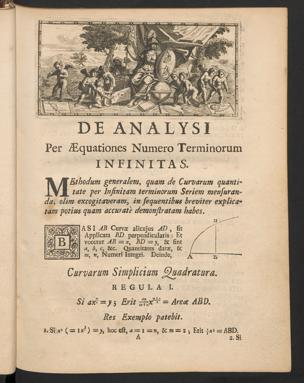
\includegraphics[width=1\textwidth]{figures/newton.jpg}\\
% \href{https://de.wikipedia.org/wiki/Datei:NewtonIteration_Ani.gif}{Link to a simple example.}
%\end{column}
%\end{columns}
%\end{frame}
%
%\begin{frame}{Deterministic simulation in Dynare}
%Keywords:
%    \begin{wideitemize}
%    \item \texttt{initval}: Sets the initial steady state
%    \item \texttt{endval}: Sets the terminal steady state
%    \item \texttt{shocks}: Specify shocks for the simulation path
%    \item \texttt{histval}: For states outside the steady state
%    \item \texttt{perfect\_foresight\_setup}; sets up the simulation
%    \item \texttt{perfect\_foresight\_solver}; run the simulations
%    \item Many options are available. See the Dynare manual.
%    \end{wideitemize}
%\end{frame}

\begin{frame}[fragile]{Perfect foresight: brute force ELB implementation}
\begin{wideitemize}
\item ELB implementation via $\max$-operator in the \texttt{model}-block.
\begin{minted}{c++}
[name='Notional rate Taylor rule']
inomnot=rhoinom*inomnot(-1)
        +(1-rhoinom)*(phi_pi*pie+phi_y*y)+zeps_i;

[name = 'Observed interest rate']
inom = max(inomnot,ilb);
\end{minted}
\item Of note: $\max$-operator is not differentiable\\
$\rightarrow$ challenging for Newton-type solvers that rely on (sparse) Jacobian
\end{wideitemize}
\end{frame}


\begin{frame}[fragile]{Simulating a demand shock of 1\%}
\begin{minted}{c++}
shockssequence = -0.01;

shocks;
    var u_c;
    periods 1;
    values(shockssequence);
end;

perfect_foresight_setup(periods=50);
perfect_foresight_solver;
\end{minted}
\begin{wideitemize}
\item Important: allow for sufficiently many periods to return back to steady state
\end{wideitemize}
\end{frame}


\begin{frame}[fragile]{Perfect foresight: mixed complementarity problem (MCP) implementation}
\begin{wideitemize}
\item Alternative: use specialized \hi{mixed complementary problem (MCP)} solver:
\begin{itemize}
\item Levenberg-Marquardt mixed complementarity problem solver \parencite{KanzowPetra2004} triggered by keyword \texttt{lmmcp} or\\
     \texttt{perfect\_foresight\_solver(stack\_solve\_algo=7, solve\_algo=10)}
\item PATH solver \parencite{FerrisMunson1999}: \\ \texttt{perfect\_foresight\_solver(stack\_solve\_algo=7, solve\_algo=11)}
\end{itemize}
\item Solvers require particular type of setup:
\begin{align}
        LB =&X  &\Rightarrow   F(X)>0,\\
       LB\leq &X \leq UB &\Rightarrow   F(X)=0,\\
        &X =UB &\Rightarrow   F(X)<0.
\end{align}
\item Sign of the equation residual with binding constraint matters
\item Convention in Dynare: LHS-RHS
\end{wideitemize}
\end{frame}

\begin{frame}[fragile]{Perfect foresight: MCP implementation}
\begin{wideitemize}
\item Explicitly specify a complementarity condition for the Taylor rule using the perpendicular symbol:
\begin{itemize}
        \item  ⟂ UTF-8 symbol (Unicode codepoint U+27C2)
        \item  \textunderscore|\textunderscore : pure ASCII, i.e. a vertical bar enclosed within two underscores
\end{itemize}
\begin{minted}{c++}
[name='Notional rate Taylor rule'] 
inom=inomnot ⟂ inom>-0.0055;

[name='Notional rate Taylor rule']
inomnot=rhoinom*inomnot(-1)
        +(1-rhoinom)*(phi_pi*pie+phi_y*y)+zeps_i;
\end{minted}
\item If lower bound on interest rate is binding
\begin{equation}
  residual=i_t-i_t^{not}>0
\end{equation}

\end{wideitemize}
\end{frame}

\begin{frame}[fragile]{Perfect foresight: MCP implementation}
\begin{wideitemize}
\item Alternative: older syntax where \texttt{mcp}-tag indicates equation to be replaced (RHS expression is not parsed!)
\begin{minted}{c++}
[name='Notional rate Taylor rule',mcp='inom>-0.0055']
inom=inomnot;

[name='Notional rate Taylor rule']
inomnot=rhoinom*inomnot(-1)
        +(1-rhoinom)*(phi_pi*pie+phi_y*y)+zeps_i;
\end{minted}
\item If lower bound on interest rate is binding
\begin{equation}
  residual=i_t-i_t^{not}>0
\end{equation}

\end{wideitemize}
\end{frame}


\begin{frame}[fragile]{Simulating a demand shock of 1\%}
\begin{minted}{c++}
shockssequence = -0.01;

shocks;
    var u_c;
    periods 1;
    values(shockssequence);
end;

perfect_foresight_setup(periods=50);
perfect_foresight_solver(lmmcp);
\end{minted}
\begin{itemize}
\item Specialized solver triggered by keyword \texttt{lmmcp}
\end{itemize}
\end{frame}

%\begin{frame}[fragile]{Pre-announced shock}
%\begin{wideitemize}
%\item Example of a pre-announced monetary policy shock
%\begin{minted}{c++}
%shockssequence = 0.01;
%
%shocks;
%var u_i;
%periods 4;
%values(shockssequence);
%end;
%
%perfect_foresight_setup(periods=300);
%perfect_foresight_solver;
%\end{minted}
%\end{wideitemize}
%\end{frame}
%
%
%
%
%\begin{frame}[fragile]{Permanent shock}
%\begin{wideitemize}
%\item Example of a permanent cost-push shock
%\begin{minted}{c++}
%initval;
%u_a = 0;
%end;
%steady ;
%
%endval;
%u_a = -0.001;
%end;
%steady;
%
%perfect_foresight_setup(periods=300);
%perfect_foresight_solver;
%\end{minted}
%\end{wideitemize}
%\end{frame}



%\begin{frame}[fragile]{Output}
%\begin{wideitemize}
%\item Dynare stores the endogenous variables $\left(x_0 \quad x_1  \quad ... x_T \quad x_{T+1}\right)$ in the field \texttt{oo\_.endo\_simul}
%\item Dynare stores the exgenous variables $\left(u_1  \quad ... u_T \right)'$ in the field \texttt{oo\_.exo\_simul}
%\end{wideitemize}
%\end{frame}
%
%
%
%\begin{frame}{Hands-on}
%\begin{wideitemize}
%\item Let's look at the \hi{code for deterministic simulations} in practice.
%\end{wideitemize}
%\end{frame} 

\section{Stochastic simulations: OccBin}

% LTeX: language=en-US

\begin{frame}{Overview}
    \begin{wideitemize}
    \item Dynare applies a \hi{perturbation} approach to solve stochastic model: Taylor expansion
	\item But: OBCs introduce non-differentiability
    \item OccBin \parencite{GuerrieriIacoviello2015}: handle OBCs using a piecewise linear approach
    \item OBCs are different regimes of the same model, e.g.:
    \begin{itemize}
        \item economy outside the ELB
        \item economy at the ELB
    \end{itemize}
    \item The solution can be highly nonlinear due to feedback loop:
	\begin{itemize}
		\item dynamics in one regime depend on its expected duration
		\item in turn, the expected duration depends on the states
		\end{itemize}
    \end{wideitemize}
\end{frame}


\begin{frame}{Strengths and weaknesses}
    \begin{wideitemize}
	\item Similar to the linear solutions, the method does not take into account uncertainty (and (precautionary) behaviour towards it)\\
	$\rightarrow$ solution does not take into account that the constraint(s) could be binding in the future (e.g. because of unrealised shocks).
	\item But:
	\begin{itemize}
		\item it is quite fast and can be used for estimation
		\item can be applied to very large models
	\end{itemize}
    \end{wideitemize}
\end{frame}

\begin{frame}{Representing two regimes}
\begin{wideitemize}
\item The reference/baseline regime (e.g.\ ELB constraint is slack) can be expressed as a linearized system:
\begin{equation}\label{eq:M1}
A_1E_t\left[X_{t+1}\right] + A_0X_t  + A_{-1}X_{t-1} +  \mathcal{E} u_t = 0 \: , \tag{M1}
\end{equation}
where $X_t$ denotes the model variables in deviation from steady state.
\item The alternative regime (e.g.\ ELB constraint is binding) features a constant $D^{\ast}$
\begin{equation}\label{eq:M2}
A_1^{\ast}E_t\left[X_{t+1}\right] + A_0^{\ast}X_t  + A_{-1}^{\ast}X_{t-1} + D^{\ast}+ \mathcal{E}^{\ast} u_t \tag{M2}
\end{equation}
\item Both models \ref{eq:M1} and \ref{eq:M2} are linearized around the same point ($D^*$ accounts for potentially different steady states)
\item Important: reference regime is the one where the system settles without any shocks
\end{wideitemize}
\end{frame}

\begin{frame}{Regimes and solutions}
\begin{columns}[T]
\column{0.5\linewidth}
\hi{Reference regime (M1)}
\begin{wideitemize}
    \item Solution can be written as:
        \begin{equation}\label{eq:M1DR}
        X_t = \mathcal{P}X_{t-1} + Cu_t \tag{M1DR}
        \end{equation}
        \item Transition matrices $\mathcal{P}$ and $C$ are constant
        \item Blanchard-Kahn conditions hold
        \item Provides linearization point
\end{wideitemize}
\column{0.5\linewidth}
\hi{Alternative regime (M2):}
\begin{wideitemize}
    \item  Solution   can be written as:
    \begin{equation}\label{eq:M2DR}
        X_t =
            \begin{cases}
            \mathcal{P}_{t}X_{t-1} + R_t + C_tu_t \, &\text{for } t = 1 \\
              \mathcal{P}_tX_{t-1} + R_t \, &\text{for } t \geq 2
            \end{cases}
            \tag{M2DR}
        \end{equation}
        \item Time-varying matrices depending on expected regime length
\end{wideitemize}
\end{columns}
\vspace{1cm}
\begin{itemize}
\item Assumes certainty equivalence: system does not depend on $u_{t+j}$ for $j \geq 1$\\
$\rightarrow$ people expect future shocks to equal their expected value of 0 with certainty
\end{itemize}
\end{frame}

\begin{frame}{Solution strategy: Backward induction + Guess and verify}
\begin{wideitemize}
\item We know terminal condition: if $u_{t} = 0$ for all future periods, system by construction returns to reference regime M1\\
$\rightarrow$ need to check whether we are indeed back in $M1$ from $T$ onwards (i.e.\ the constraint is slack)
\item For $t<T$: Regime M2 given state $X_{t-1}$ (and potentially shocks $u_t$)
\item Guess and verify approach to find regime length:
\begin{wideenumerate}
	\item Guess $T$ in period $t_0$ such that for $t \geq T$, we are back in $M1$
	\item Check whether guess is consistent with implied model dynamics
	\item If not, update guess
\end{wideenumerate}
\end{wideitemize}
\end{frame}

\begin{frame}{Working backwards: the terminal period $T$}
\begin{wideitemize}
\item For any $t \geq T$ with expected $u_t=0$, the solution in regime $M1$, \eqref{eq:M1DR}, implies:
\begin{equation}
X_{t} = \mathcal{P}X_{t-1}
\end{equation}
\item For expectations in $T-1$ then follows:
\begin{equation}
E_{T-1}\left[X_{T}\right]=\mathcal{P}X_{T-1}
\end{equation}
\item This allows eliminating the forward-looking part of the linear system for $M2$:
\begin{equation}
\begin{split}
A_1^{\ast}E_{T-1}\left[X_{T}\right] + A_0^{\ast}X_{T-1}  + A_{-1}^{\ast}X_{T-2} + D^{\ast}&=\\
A_1^{\ast}{\color{blue}\mathcal{P}X_{T-1}} + A_0^{\ast}X_{T-1}  + A_{-1}^{\ast}X_{T-2} + D^{\ast}&= 0
  \end{split}
\end{equation}
\item Given inherited states $X_{T-2}$, this is a matrix equation in one unknown: $X_{T-1}$
\end{wideitemize}
\end{frame}

\begin{frame}{Working backwards: the solution for $T-1$}
\begin{wideitemize}
\item Solve for $X_{T-1}$ given $X_{T-2}$ to get the decision rule:
\begin{equation}
  X_{T-1} = -\left(A_1^{\ast}\mathcal{P}+A_0^{\ast}\right)^{-1}\left(A_{-1}^{\ast}X_{T-2}+D^{\ast}\right)
\end{equation}
\item Looks complicated, but is actually linear:
\begin{equation}
  X_{T-1} =  \underbrace{\mathcal{P}_{T-1}}_{-\left(A_1^{\ast}\mathcal{P}+A_0^{\ast}\right)^{-1}A_{-1}^{\ast}}X_{T-2}
  + \underbrace{R_{T-1}}_{-\left(A_1^{\ast}\mathcal{P}+A_0^{\ast}\right)^{-1}D^{\ast}}
\end{equation}
\item Linearity allows for easy evaluation of conditional expectations $E_{T-2}[X_{T-1}]$ required in $T-2$
\end{wideitemize}
\end{frame}

\begin{frame}{Working backwards until the first period}
\begin{wideitemize}
\item Continue the drill with the previous period $T-2$:
\begin{equation}
  A_1^{\ast}\mathcal{P}_{T-1}X_{T-2} + A_0^{\ast}X_{T-2}  + A_{-1}^{\ast}X_{T-3} + D^{\ast}= 0
\end{equation}
\item Solve for $X_{T-2}$ given $X_{T-3}$ to get the decision rule:
\begin{equation}
	X_{T-2} =    \mathcal{P}_{T-2}X_{T-3}+ R_{T-2}
\end{equation}
with
\begin{align}
\mathcal{P}_{T-2} &= -\left(A_1^{\ast}\mathcal{P}_{T-1}+A_0^{\ast}\right)^{-1}A_{-1}^{\ast}\\
R_{T-2} &= -\left(A_1^{\ast}\mathcal{P}_{T-1}+A_0^{\ast}\right)^{-1}D^{\ast}
\end{align}
\item $\mathcal{P}_t, R_t$ and later $C_t$ are time-varying matrices composed of structural matrices in M1 and M2\\
$\rightarrow$ nonlinear dynamics
\end{wideitemize}
\end{frame}

\begin{frame}{Working backwards: the first period}
\begin{wideitemize}
\item We finally reach the first period $t=1$:
\begin{equation}
  A_1^{\ast}\mathcal{P}_{2}X_{1} + A_0^{\ast}X_{1}  + A_{-1}^{\ast}X_{0} + D^{\ast}+ \mathcal{E}^{\ast} u_1= 0
\end{equation}
\item Solve for $X_{1}$ given $X_{0}$ and current shock $u_1$ to get the decision rule:
\begin{equation}
	X_{1} =    \mathcal{P}_{1}X_{0}+ R_{1}+C_1 u_1
\end{equation}
with
\begin{align}
\mathcal{P}_{1} &= -\left(A_1^{\ast}\mathcal{P}_{2}+A_0^{\ast}\right)^{-1}A_{0}^{\ast}\\
R_{1} &= -\left(A_1^{\ast}\mathcal{P}_{2}+A_0^{\ast}\right)^{-1}D^{\ast}\\
C_{1} &= -\left(A_1^{\ast}\mathcal{P}_{2}+A_0^{\ast}\right)^{-1}\mathcal{E}^{\ast}
\end{align}
\item This completes the computation of the solution \eqref{eq:M2DR}
\end{wideitemize}
\end{frame}


\begin{frame}{Verification}
\begin{wideitemize}
\item We now have obtained time-dependent decision rules for all periods, but conditional on potentially wrongly guessed $T$\\
\item Is behavior of economy starting from $X_0$ with given shock $\varepsilon_1$ consistent with conjectured decision rules?\\
$\rightarrow$  compute (time) path for $X_{t+j}$ and implied reversal to the baseline regime $\tilde T$
\item If $\tilde T =T$ is verified: we have found a solution!
\item If not, update the guess for the regime sequence and back to square one
	\begin{itemize}
		\item Make use of the computed path for $X_t$ to update the next guess (default)
		\item Other updating schemes are possible (e.g.\ step-wise changes of the regime guess:\\ \texttt{simul\_curb\_retrench})
	\end{itemize}
\item Multiple solutions: multiple regime sequences possible \parencite{Holden2022}
\end{wideitemize}
\end{frame}


\begin{frame}[fragile]{OccBin model block}
\begin{wideitemize}
\item Equation \texttt{name} tags are used to name equations
\item \texttt{bind} and \texttt{relax}-tags assign equation pairs to the alternative and the reference regime, respectively, associated with the constraint named \texttt{zlb}
\begin{minted}{c++}
[name='Notional rate Taylor rule']
inomnot=(1-rhoinom)*inomnot(-1)
        +rhoinom*(phi_pi*pie+phi_y*y)+zeps_i;

[name = 'Observed interest rate',relax='zlb']
inom = inomnot;

[name = 'Observed interest rate',bind='zlb']
inom = ilb;
\end{minted}
\end{wideitemize}
\end{frame}

\begin{frame}[fragile]{OccBin constraints definition}
\begin{wideitemize}
\item Declare regime switching condition
\begin{minted}{c++}
occbin_constraints;
name 'zlb'; bind inomnot<=ilb;
end;
\end{minted}
which is equivalent to
\begin{minted}{c++}
occbin_constraints;
name 'zlb'; bind inomnot<=ilb; relax inomnot>ilb;
end;
\end{minted}
\item Explicit \texttt{relax}-tags are required when \texttt{bind}-expression cannot be evaluated in alternative regime
\end{wideitemize}
\end{frame}



\begin{frame}[fragile]{OccBin constraints: numerical considerations}
\begin{wideitemize}
\item In each simulation period, Dynare will check the respective conditions to see whether a regime change takes place\\
    $\rightarrow$ numerical imprecisions can cause spurious changes at the boundary between regimes
\item Useful trick: introducing a safety buffer:
\begin{minted}{c++}
occbin_constraints;
name 'zlb'; bind inomnot<=ilb-1e-8; relax inomnot>ilb+1e-8;
end;
\end{minted}
\end{wideitemize}
\end{frame}

\begin{frame}[fragile]{Defining surprise shocks}
\begin{minted}{c++}
shockssequence = -0.01;

shocks(surprise);
    var u_c;
    periods 1;
    values(shockssequence);
end;
\end{minted}
\begin{wideitemize}
  \item Keyword \texttt{surprise} of \texttt{shocks}-block indicates that perfect foresight syntax is used, but future shocks are not anticipated
\end{wideitemize}
\end{frame}

\begin{frame}[fragile]{Triggering OccBin simulations}
\begin{minted}{c++}
occbin_setup; //instruct OccBin use
occbin_solver(simul_periods=20,simul_check_ahead_periods=50);
occbin_graph y inom inomnot pie;
\end{minted}
\begin{wideitemize}
  \item \texttt{occbin\_setup} is mandatory to trigger the use of the OccBin toolkit (translates\\ \texttt{shocks(surprise)-block})
  \item \texttt{occbin\_solver} triggers actual simulation run
  \begin{itemize}
    \item \texttt{simul\_periods}: number of periods for which to compute simulation
    \item \texttt{simul\_check\_ahead\_periods}: initial guess for period $T$ at which regime returns to baseline
  \end{itemize}
\end{wideitemize}
\end{frame}

\begin{frame}{OccBin output}
\begin{wideitemize}
\item Dynare stores all OccBin simulation-related output in \texttt{oo\_.occbin.simul}
\begin{wideitemize}
  \item the simulated solution paths in \texttt{oo\_.occbin.simul.endo\_piecewise}
  \item the linear simulation when ignoring the constraints in \texttt{oo\_.occbin.simul.endo\_linear}
  \item an error-flag in \texttt{oo\_.occbin.simul.error\_flag}
  \item the regime and its expected duration in \texttt{oo\_.occbin.simul.regime\_history}
\end{wideitemize}
\item Details can be found in the manual
\end{wideitemize}
\end{frame}

\begin{frame}{OccBin: nonlinear models}
\begin{wideitemize}
\item Dynare's implementation can handle non-linearly entered models\\
$\rightarrow$ Dynare will do the linearization
\item Attention: expressions within \texttt{occbin\_constraints}-block are not linearized (yet)\\
$\rightarrow$ risk for inconsistency
\end{wideitemize}
\end{frame}

%\begin{frame}{Hands-on}
%\begin{wideitemize}
%\item Let's look at the \hi{code for OccBin simulations} in practice.
%\end{wideitemize}
%\end{frame}
%
%\subsection{OBCs with Kuhn-Tucker constraints}
%\begin{frame}{Bonus: Kuhn-Tucker}
%\begin{wideitemize}
%\item The ELB constraint was relatively easy to implement. The lower bound does not contain choice  variables.
%\item Now we consider the model used in \textcite{cuba2019likelihood}
%\item This model with endogenous borrowing constraints can be cast into a Kuhn-Tucker framework
%\item It is the core of many modern macro models with nonlinearities such as Mendoza (2006), Bocola
%(2016), and He and Krishnamurthy (2011).
%\end{wideitemize}
%\end{frame}
%
%
%\begin{frame}{Consumption savings under borrowing constraints}
%\begin{wideitemize}
%\item A consumer maximises utility from consumption $C_t$
%\begin{equation*}
%    \max E_0 \sum_{t=0}^{\infty}\beta^t\frac{C^{1-\gamma}}{1-\gamma}
%\end{equation*}
%subject to the budget constraint:
%\begin{equation*}
%    C_t + RB_{t-1} = Y_t + B_t
%\end{equation*}
%with gross interest rate $R$ and a constraint on borrowing $B_t$ with attached multiplier $\lambda_t$
%\begin{equation*}
%    B_t \leq mY_t
%\end{equation*}
%\item Income is stochastic:
%\begin{equation*}
%    \log(Y_t) = \rho \log(Y_{t-1})+ \sigma \varepsilon_t.
%\end{equation*}
%\end{wideitemize}
%\end{frame}
%
%\begin{frame}{Equilibrium}
%\begin{wideitemize}
%\item Intertemporal consumption optimality:
%\begin{equation*}
%  C_t^{-\gamma} = \beta R E_t\left[C_{t+1}^{-\gamma}\right]+\lambda_t
%\end{equation*}
%\item A Kuhn-Tucker condition ($\lambda_t$ gives the value of relaxing the borrowing constraint):
%\begin{equation*}
%    \lambda_t \left(B_t-mY_t\right)=0
%\end{equation*}
%\begin{itemize}
%\item If income and assets are low: Borrowing constraint (more likely) binds
%\item If income and assets are high: Borrowing can be relatively high relative to future consumption even if borrowing remains below the maximum allowed.
%\end{itemize}
%\item For higher-than-average income realisations, consumption is
%sufficiently high today relative to the future that it is optimal to save for the future.
%\item The borrowing constraint
%becomes temporarily slack ($\lambda_t > 0$).
%\end{wideitemize}
%\end{frame}
%
%\begin{frame}[fragile]{Bringing the model into the computer}
%\smartdiagramset{back arrow disabled,module minimum width=2.cm,font=\footnotesize}
%\smartdiagram[flow diagram:horizontal]{Preamble, Model definition, Steady state, Simulation and estimation}
%\end{frame}
%
%
%\begin{frame}[fragile]{Preamble}
%\begin{columns}
%\begin{column}[T]{0.4\textwidth}
%	    \begin{wideitemize}
%	        \item Endogenous variables: $B_t, C_t, Y_t, \lambda_t$
%	        \item Exogenous variables (shocks): $\varepsilon_t$
%	        \item Parameters: $ \beta, \gamma, m, \rho, R, \sigma$
%	        \item We take the calibration from Cuba-Borda et al. (2019)
%	    \end{wideitemize}
%\end{column}
%\begin{column}[T]{0.6\textwidth}
%\begin{minted}{c++}
%var b  c lam y ;
%varexo u_u ;
%parameters BETA, M, R, RHO,
%SIG, GAMMAC;
%
%BETA = 0.945;
%GAMMAC = 1;
%RHO   = 0.9;
%R = 1.05;
%SIG = 0.01;
%M = 1;
%\end{minted}
%\end{column}
%\end{columns}
%\end{frame}
%
%\begin{frame}[fragile]{Model definition}
%\begin{columns}
%\begin{column}[T]{0.35\textwidth}
%	    \begin{wideitemize}
%	        \item $C_t  = Y_t + B_t -RB_{t-1}$
%	        \item $C_t^{-\gamma} = \beta R E_t\left[C_{t+1}^{-\gamma}\right]+\lambda_t$
%	        \item $\log(Y_t) = \rho \log(Y_{t-1})+ \sigma \varepsilon_t$
%	        \item $\lambda_t \left(B_t-mY_t\right)=0$
%	    \end{wideitemize}
%\end{column}
%\begin{column}[T]{0.65\textwidth}
%\begin{minted}{c++}
%model;
%[name = 'Budget constraint']
%c = y + b - R*b(-1) ; //
%[name = 'Euler equation']
%1/c^GAMMAC = BETA*R/c(+1)^GAMMAC + lam ;
%[name = 'Stochastic income']
%log(y) = RHO*log(y(-1)) + SIG*eps_u;
%[name = 'KT-constraint', relax='BORRCON']
%(b -  M*y) = 0 ;  //
%[name = 'KT-constraint', bind='BORRCON']
%lam = 0 ;
%end;
%\end{minted}
%\end{column}
%\end{columns}
%\end{frame}
%
%\begin{frame}[fragile]{Steady state}
%\begin{columns}
%\begin{column}[T]{0.4\textwidth}
%	    \begin{wideitemize}
%	        \item Based on a unit income, we can find the steady state.
%	        \item The household is borrowing constrained.
%	        \item Consumption equals income minus the steady-state debt service cost.
%	    \end{wideitemize}
%\end{column}
%\begin{column}[T]{0.6\textwidth}
%\begin{minted}{c++}
%steady_state_model;
%b=M;
%y=1;
%c=y+M-R*M;
%lam=(1-BETA*R)/c^GAMMAC;
%end;
%\end{minted}
%\end{column}
%\end{columns}
%\end{frame}
%
%\begin{frame}[fragile]{Declare OBCs}
%\begin{minted}{c++}
%occbin_constraints;
%name 'BORRCON'; bind lam < 0; relax b > M*y;
%end;
%\end{minted}
%\begin{itemize}
%    \item Trick: Define constraint in terms of $\lambda$.
%    \item The rest of the simulation is coded up for you in the examples.
%\end{itemize}
%\end{frame}
%
%\begin{frame}{Hands-on}
%\begin{wideitemize}
%\item Let's look at the \hi{code for OccBin simulations} for this model.
%\end{wideitemize}
%\end{frame} 

%
%\begin{frame}{Deterministic and stochastic simulations}
	\begin{itemize}
%	    \item In general, we are interested in using our model for policy experiments and other simulations.
%	    \begin{itemize}
%	        \item How do agents react to temporary or permanent shocks?
%	    \end{itemize}
	    \item Dynare offers \hi{two ways} to solve and simulate the model:
	    \begin{enumerate}
            \item \hi{Deterministic} simulations (perfect foresight):  all future shocks are known exactly.
	       \item \hi{Stochastic} simulations (perturbation):  only the shock distributions are known.
        \end{enumerate}
%	   \item We will build some intuition on how Dynare performs these simulations.
%         \begin{itemize}
%	        \item We also consider OccBin - a toolkit to simulate models with OBCs
%	    \end{itemize}
%	    %\item There are other methods, such as projection methods, which I will not discuss.
%	\end{wideitemize}
%\end{frame}
%
%\begin{frame}{Deterministic and stochastic simulations (cont'd)}
%	\begin{wideitemize}
%	    \item Dynare translates your model into a general form.\footnote{A great intro by Willi Mutschler: \url{https://www.youtube.com/watch?v=KHTEZiw9ukU}}
%	    \item Let $x_t$ denote the vector of endogenous variables at time $t$, $u_t$ the shocks (at the beginning of the period) and $\theta$ the parameters.
%	    \item Deterministic (no uncertainty) $f\left(x_{t-1},x_t,x_{t+1},u_t | \theta \right)$
%          \item Stochastic (with shocks) $Ef\left(x_{t-1},x_t,x_{t+1},u_t | \theta \right) =0,$ with decision rules $x_t = g(x_{t-1},u_t|\theta)$ and assumptions about shock distributions.
%	\end{wideitemize}
%\end{frame}
%
%\begin{frame}{Deterministic and stochastic simulations (cont'd)}
\item Both employ different techniques and have different advantages and limitations.
\begin{columns}[T]
\column{0.5\linewidth}
\begin{wideitemize}
    \item \hi{Deterministic:}
     \begin{itemize}
	        \item[+] Arbitrary precision
	        \item[+] Easily captures nonlinearities (such as OBCs)
	        \item[-] Assumptions of perfect foresight
	        \item[-] How to simulate time series?
	    \end{itemize}
\end{wideitemize}
\column{0.5\linewidth}
\begin{wideitemize}
    \item \hi{Stochastic:}
	      \begin{itemize}
	        \item[+] Captures uncertainty
	        \item[+] Needed for estimation with state space form
	        \item[-] Often uses 1st order approximations: Certainty equivalence
	        \item[-] High-order approximations are possible but can be challenging to use for OBCs
	        \item[+] Perturbation methods can capture OBCs with additional tools (OccBin)
	    \end{itemize}
\end{wideitemize}
\end{columns}
\end{itemize}
\end{frame}


\begin{frame}{Our plan on simulations}
\begin{wideenumerate}
    \item Deterministic simulations: Method and example with OBCs
    \item Stochastic simulations: Method and example
    \item Occbin simulations: Method and example with OBCs
\end{wideenumerate}
\end{frame}




\section{Deterministic simulations}
%\begin{frame}{Our NKM in the general deterministic framework}
%	\begin{wideitemize}
%	\item General deterministic model: $f\left(x_{t-1},x_t,x_{t+1},u_t | \theta \right)$
%	    \item Our model:
%	    \begin{align*}
%	        x_t &= \left(\pi_t \quad y_t \quad i_t \quad \cdots\right)'\\
%	           u_t &= \left(u^a_t \quad u^c_t \quad  u^i_t\right)'
%	    \end{align*}
%        \item Thus (omitting the shock processes):
%       \begin{align*}
%        f\left(x_{t-1},x_t,x_{t+1},u_t | \theta \right) =
%            \begin{pmatrix}
%                \pi_t - \beta E_t\left[\pi_{t+1}\right]-\kappa y_t- \varepsilon_t^a  \\
%                y_t -E_t \left[y_{t+1} \right]+ \frac{1}{\sigma}\left(i_t-E_t\left[\pi_{t+1}\right]\right)-\varepsilon_t^c  \\
%                i_t - \phi_\pi \pi_t - \phi_y y_t-\varepsilon_t^i \\
%                \vdots
%            \end{pmatrix}
%        \end{align*}
%    \end{wideitemize}
%\end{frame}
%
%
%\begin{frame}{Model solution: Stacked system}
%    \begin{wideitemize}
%    \item Dynare solves a stacked system of nonlinear difference equations:\footnote{\url{https://stephane-adjemian.fr/dynare/slides/perfect-foresight-models.pdf}}
%    \begin{align*}
%    f\left(x_{2},x_{1},{\color{red}x_{0}},u_{1}\right) &= 0\\
%    f\left(x_{3},x_{2},x_{1},u_{2}\right) &= 0\\
%    \vdots \\
%    f\left(x_{t+1},x_{t},x_{t-1},u_{t}\right) &= 0\\
%    \vdots \\
%    f\left({\color{red}x_{T+1}},x_{T},x_{T},u_{T}\right) &= 0
%    \end{align*}
%    \item Compact notation: $F\left(\boldsymbol{X}\right) = 0$ with $\boldsymbol{X} = [x_1',x_2',...,x_T']'$, i.e. the entire solution path.
%    \item Boundary conditions: $x_0$ and $x_{T+1}$
%    \end{wideitemize}
%\end{frame}
%
%\begin{frame}{Numerical approach: Newton algorithm}
%\begin{columns}
%    \begin{column}[T]{0.8\textwidth}
%	    \begin{itemize}
%	        \item Start an initial guess $\boldsymbol{X^{(0)}}$
%	        \item Update the trajectories (solution paths) by iterating ($i = 0.1,...$) and solving:
%	        \begin{equation*}
%	           F\left(\boldsymbol{X}^{i+1}\right) =   J_F\left(\boldsymbol{X}^{i+1}\right)\left( \boldsymbol{X}^{(i+1)}-\boldsymbol{X}^{(i)}\right)
%	        \end{equation*}
%	        where $J_F\left(\boldsymbol{X}^{i+1}\right)$ is the Jacobian matrix of partial derivatives of $F()$.
%	        \item Stop if
%	         \begin{equation*}
%	           || F\left(\boldsymbol{X}^{i+1}\right) || < crit.
%	        \end{equation*}
%	        \item Lot's of room for improvement:
%	        \begin{itemize}
%    	        \item The size of $J_F$: Exploit sparsity and triangular model structure.
%    	       \item Optimise step size
%	        \end{itemize}
%	    \end{itemize}
%\end{column}
%\begin{column}[T]{0.2\textwidth}
%
%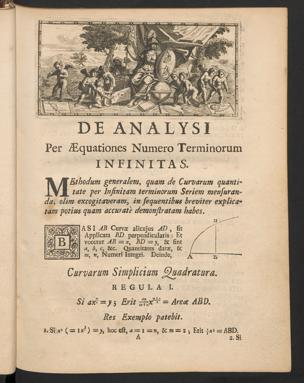
\includegraphics[width=1\textwidth]{figures/newton.jpg}\\
% \href{https://de.wikipedia.org/wiki/Datei:NewtonIteration_Ani.gif}{Link to a simple example.}
%\end{column}
%\end{columns}
%\end{frame}
%
%\begin{frame}{Deterministic simulation in Dynare}
%Keywords:
%    \begin{wideitemize}
%    \item \texttt{initval}: Sets the initial steady state
%    \item \texttt{endval}: Sets the terminal steady state
%    \item \texttt{shocks}: Specify shocks for the simulation path
%    \item \texttt{histval}: For states outside the steady state
%    \item \texttt{perfect\_foresight\_setup}; sets up the simulation
%    \item \texttt{perfect\_foresight\_solver}; run the simulations
%    \item Many options are available. See the Dynare manual.
%    \end{wideitemize}
%\end{frame}

\begin{frame}[fragile]{Perfect foresight: brute force ELB implementation}
\begin{wideitemize}
\item ELB implementation via $\max$-operator in the \texttt{model}-block.
\begin{minted}{c++}
[name='Notional rate Taylor rule']
inomnot=rhoinom*inomnot(-1)
        +(1-rhoinom)*(phi_pi*pie+phi_y*y)+zeps_i;

[name = 'Observed interest rate']
inom = max(inomnot,ilb);
\end{minted}
\item Of note: $\max$-operator is not differentiable\\
$\rightarrow$ challenging for Newton-type solvers that rely on (sparse) Jacobian
\end{wideitemize}
\end{frame}


\begin{frame}[fragile]{Simulating a demand shock of 1\%}
\begin{minted}{c++}
shockssequence = -0.01;

shocks;
    var u_c;
    periods 1;
    values(shockssequence);
end;

perfect_foresight_setup(periods=50);
perfect_foresight_solver;
\end{minted}
\begin{wideitemize}
\item Important: allow for sufficiently many periods to return back to steady state
\end{wideitemize}
\end{frame}


\begin{frame}[fragile]{Perfect foresight: mixed complementarity problem (MCP) implementation}
\begin{wideitemize}
\item Alternative: use specialized \hi{mixed complementary problem (MCP)} solver:
\begin{itemize}
\item Levenberg-Marquardt mixed complementarity problem solver \parencite{KanzowPetra2004} triggered by keyword \texttt{lmmcp} or\\
     \texttt{perfect\_foresight\_solver(stack\_solve\_algo=7, solve\_algo=10)}
\item PATH solver \parencite{FerrisMunson1999}: \\ \texttt{perfect\_foresight\_solver(stack\_solve\_algo=7, solve\_algo=11)}
\end{itemize}
\item Solvers require particular type of setup:
\begin{align}
        LB =&X  &\Rightarrow   F(X)>0,\\
       LB\leq &X \leq UB &\Rightarrow   F(X)=0,\\
        &X =UB &\Rightarrow   F(X)<0.
\end{align}
\item Sign of the equation residual with binding constraint matters
\item Convention in Dynare: LHS-RHS
\end{wideitemize}
\end{frame}

\begin{frame}[fragile]{Perfect foresight: MCP implementation}
\begin{wideitemize}
\item Explicitly specify a complementarity condition for the Taylor rule using the perpendicular symbol:
\begin{itemize}
        \item  ⟂ UTF-8 symbol (Unicode codepoint U+27C2)
        \item  \textunderscore|\textunderscore : pure ASCII, i.e. a vertical bar enclosed within two underscores
\end{itemize}
\begin{minted}{c++}
[name='Notional rate Taylor rule'] 
inom=inomnot ⟂ inom>-0.0055;

[name='Notional rate Taylor rule']
inomnot=rhoinom*inomnot(-1)
        +(1-rhoinom)*(phi_pi*pie+phi_y*y)+zeps_i;
\end{minted}
\item If lower bound on interest rate is binding
\begin{equation}
  residual=i_t-i_t^{not}>0
\end{equation}

\end{wideitemize}
\end{frame}

\begin{frame}[fragile]{Perfect foresight: MCP implementation}
\begin{wideitemize}
\item Alternative: older syntax where \texttt{mcp}-tag indicates equation to be replaced (RHS expression is not parsed!)
\begin{minted}{c++}
[name='Notional rate Taylor rule',mcp='inom>-0.0055']
inom=inomnot;

[name='Notional rate Taylor rule']
inomnot=rhoinom*inomnot(-1)
        +(1-rhoinom)*(phi_pi*pie+phi_y*y)+zeps_i;
\end{minted}
\item If lower bound on interest rate is binding
\begin{equation}
  residual=i_t-i_t^{not}>0
\end{equation}

\end{wideitemize}
\end{frame}


\begin{frame}[fragile]{Simulating a demand shock of 1\%}
\begin{minted}{c++}
shockssequence = -0.01;

shocks;
    var u_c;
    periods 1;
    values(shockssequence);
end;

perfect_foresight_setup(periods=50);
perfect_foresight_solver(lmmcp);
\end{minted}
\begin{itemize}
\item Specialized solver triggered by keyword \texttt{lmmcp}
\end{itemize}
\end{frame}

%\begin{frame}[fragile]{Pre-announced shock}
%\begin{wideitemize}
%\item Example of a pre-announced monetary policy shock
%\begin{minted}{c++}
%shockssequence = 0.01;
%
%shocks;
%var u_i;
%periods 4;
%values(shockssequence);
%end;
%
%perfect_foresight_setup(periods=300);
%perfect_foresight_solver;
%\end{minted}
%\end{wideitemize}
%\end{frame}
%
%
%
%
%\begin{frame}[fragile]{Permanent shock}
%\begin{wideitemize}
%\item Example of a permanent cost-push shock
%\begin{minted}{c++}
%initval;
%u_a = 0;
%end;
%steady ;
%
%endval;
%u_a = -0.001;
%end;
%steady;
%
%perfect_foresight_setup(periods=300);
%perfect_foresight_solver;
%\end{minted}
%\end{wideitemize}
%\end{frame}



%\begin{frame}[fragile]{Output}
%\begin{wideitemize}
%\item Dynare stores the endogenous variables $\left(x_0 \quad x_1  \quad ... x_T \quad x_{T+1}\right)$ in the field \texttt{oo\_.endo\_simul}
%\item Dynare stores the exgenous variables $\left(u_1  \quad ... u_T \right)'$ in the field \texttt{oo\_.exo\_simul}
%\end{wideitemize}
%\end{frame}
%
%
%
%\begin{frame}{Hands-on}
%\begin{wideitemize}
%\item Let's look at the \hi{code for deterministic simulations} in practice.
%\end{wideitemize}
%\end{frame} 

%\subsection{Stochastic simulations}
%\begin{frame}{Stochastic simulations}
    \begin{wideitemize}
    \item Stochastic (with shocks) $Ef\left(x_{t-1},x_t,x_{t+1},u_t | \theta \right) =0,$ with decision rules $x_t = g(x_{t-1},u_t|\theta)$ and assumptions about shock distributions.
    \item Here, we search for decision functions: $g\left(\cdot\right)$ is unknown and can only be solved analytically in a few very simple cases.
    \item Dynare applies a \hi{perturbation} approach to solve model: A Taylor expansion of the original model can be used to obtain a Taylor expansion of the solution.
    \item To obtain the decision rules or policy function:
    \begin{equation*}
        x_t - x_0 = A\left(x_{t-1}-x_0\right)+Bu_t
    \end{equation*}
    \end{wideitemize}
\end{frame}

\begin{frame}[fragile]{Linearisation}
    \begin{wideitemize}
    \item We have linearised our three-equation model by hand.
    \begin{itemize}
        \item Declare the model as linear.
        \begin{minted}{c++}
        model(linear);
        \end{minted}
    \end{itemize}
    \item Dynare can linearise the model for you! Use it if you can.
    \item The model needs to be stationary to allow for linearisation around the steady state
     \begin{itemize}
        \item Dynare can handle deterministic and stochastic trends.
        \item One can always add trends back to the model.
    \end{itemize}
    \item Always (try to) provide an analytical steady state. However, Dynare can numerically solve for it based on some starting value (\texttt{initval;}).
    \end{wideitemize}
\end{frame}


\begin{frame}{Our model}
\begin{align*}
y_t 	=& E_t \left[y_{t+1} \right]- \frac{1}{\sigma}\left(i_t-E_t\left[\pi_{t+1}\right]\right)+\varepsilon_t^c \\
\pi_t 	=& \beta E_t\left[\pi_{t+1}\right]+\kappa y_t +\varepsilon_t^a \\
i_t 	=& \phi_\pi \pi_t + \phi_y y_t + \varepsilon_t^i
\end{align*}
in matrix form
\begin{equation*}
\underbrace{
\begin{bmatrix}
-1 & -1 & 0\\
-0 & \beta & 0 \\
0 & 0 & 0
\end{bmatrix}}_{A_1}
\underbrace{
\begin{bmatrix}
E_t\left[y_{t+1} \right]\\
E_t\left[\pi_{t+1} \right]\\
E_t\left[i_{t+1} \right]
\end{bmatrix}}
_{E_t[X_{t+1}]}
=
\underbrace{
\begin{bmatrix}
-1 & 0 & -\frac{1}{\sigma}\\
\kappa & -1 & 0 \\
\phi_y&\phi_\pi & -1
\end{bmatrix}}_{A_0}
\underbrace{
\begin{bmatrix}
y_{t}\\
\pi_{t}\\
i_{t}
\end{bmatrix}}_{X_t}
+\underbrace{
\begin{bmatrix}
1 & 0 & 0\\
0 & 1 & 0\\
0 & 0 & 1
\end{bmatrix}}_{\mathcal{E}}
\underbrace{
\begin{bmatrix}
\varepsilon^c_{t}\\
\varepsilon^a_{t}\\
\varepsilon^i_{t}
\end{bmatrix}}_{u_t}
\end{equation*}
\begin{itemize}
    \item Note: We used a slightly different notation by including the shock processes in matrix $\mathcal{E}$. In Dynare, $u_t$ contains only the white noise for stochastic variables, i.e. our $u$'s.
\end{itemize}
\end{frame}

\begin{frame}{How to solve the model (linearly)}
\begin{wideitemize}
\item We have a system of the form
\begin{equation*}
A_1E_t\left[X_{t+1}\right] + A_0X_t  + A_{-1}X_{t-1} +  \mathcal{E} u_t = 0
\end{equation*}
where in our case $A_{-1}$ is a matrix of zeros.
\item There are many algorithms to solve this system.
\item Dynare uses a generalised Schur decomposition based on the method of Klein (2000)\footcite{klein2000using} to obtain the solution of the form:
\begin{equation*}
    X_{t} = TX_{t-1}+Cu_t
\end{equation*}
\item Villemot (2011) shows you the algebra.\footcite{villemot2011solving}
\end{wideitemize}
\end{frame}


\begin{frame}[fragile]{Stochastic simulation command}
    \begin{wideitemize}
    \item The command  Simulates data from the model and performs IRFs \href{https://www.dynare.org/manual/the-model-file.html?highlight=stoch_sim#stoch_simul}{\texttt{stoch\_sim}}
    computes a Taylor approximation around the steady state.
    \item \texttt{order} sets the approximation order.
    \item \texttt{period} sets the number of simulation periods
    \item You can select variables to be plotted and printed on the screen.
    \begin{minted}{c++}
    stoch_simul(irf=20, order=1,periods=100) y;
    \end{minted}
    \item The Dynare reference manual lays out the many available options.
    \end{wideitemize}
\end{frame}

\begin{frame}{Accessing results}
\begin{wideitemize}
\item You can access the results of the solution (decision rules) in the results structure \texttt{oo\_.dr}
\item Field \texttt{ys} contains the steady state.
\item Field \texttt{ghx} contains the transition matrix (with all endogenous variables in deviation from the steady state)
\item Field \texttt{ghu} contains the matrix attached to the exogenous shocks
\end{wideitemize}
\end{frame}


\begin{frame}{Hands-on}
\begin{wideitemize}
\item Let's look at the \hi{code for stochastic simulations} in practice.
\end{wideitemize}
\end{frame} 

\section{Occbin}

% LTeX: language=en-US

\begin{frame}{Overview}
    \begin{wideitemize}
    \item Dynare applies a \hi{perturbation} approach to solve stochastic model: Taylor expansion
	\item But: OBCs introduce non-differentiability
    \item OccBin \parencite{GuerrieriIacoviello2015}: handle OBCs using a piecewise linear approach
    \item OBCs are different regimes of the same model, e.g.:
    \begin{itemize}
        \item economy outside the ELB
        \item economy at the ELB
    \end{itemize}
    \item The solution can be highly nonlinear due to feedback loop:
	\begin{itemize}
		\item dynamics in one regime depend on its expected duration
		\item in turn, the expected duration depends on the states
		\end{itemize}
    \end{wideitemize}
\end{frame}


\begin{frame}{Strengths and weaknesses}
    \begin{wideitemize}
	\item Similar to the linear solutions, the method does not take into account uncertainty (and (precautionary) behaviour towards it)\\
	$\rightarrow$ solution does not take into account that the constraint(s) could be binding in the future (e.g. because of unrealised shocks).
	\item But:
	\begin{itemize}
		\item it is quite fast and can be used for estimation
		\item can be applied to very large models
	\end{itemize}
    \end{wideitemize}
\end{frame}

\begin{frame}{Representing two regimes}
\begin{wideitemize}
\item The reference/baseline regime (e.g.\ ELB constraint is slack) can be expressed as a linearized system:
\begin{equation}\label{eq:M1}
A_1E_t\left[X_{t+1}\right] + A_0X_t  + A_{-1}X_{t-1} +  \mathcal{E} u_t = 0 \: , \tag{M1}
\end{equation}
where $X_t$ denotes the model variables in deviation from steady state.
\item The alternative regime (e.g.\ ELB constraint is binding) features a constant $D^{\ast}$
\begin{equation}\label{eq:M2}
A_1^{\ast}E_t\left[X_{t+1}\right] + A_0^{\ast}X_t  + A_{-1}^{\ast}X_{t-1} + D^{\ast}+ \mathcal{E}^{\ast} u_t \tag{M2}
\end{equation}
\item Both models \ref{eq:M1} and \ref{eq:M2} are linearized around the same point ($D^*$ accounts for potentially different steady states)
\item Important: reference regime is the one where the system settles without any shocks
\end{wideitemize}
\end{frame}

\begin{frame}{Regimes and solutions}
\begin{columns}[T]
\column{0.5\linewidth}
\hi{Reference regime (M1)}
\begin{wideitemize}
    \item Solution can be written as:
        \begin{equation}\label{eq:M1DR}
        X_t = \mathcal{P}X_{t-1} + Cu_t \tag{M1DR}
        \end{equation}
        \item Transition matrices $\mathcal{P}$ and $C$ are constant
        \item Blanchard-Kahn conditions hold
        \item Provides linearization point
\end{wideitemize}
\column{0.5\linewidth}
\hi{Alternative regime (M2):}
\begin{wideitemize}
    \item  Solution   can be written as:
    \begin{equation}\label{eq:M2DR}
        X_t =
            \begin{cases}
            \mathcal{P}_{t}X_{t-1} + R_t + C_tu_t \, &\text{for } t = 1 \\
              \mathcal{P}_tX_{t-1} + R_t \, &\text{for } t \geq 2
            \end{cases}
            \tag{M2DR}
        \end{equation}
        \item Time-varying matrices depending on expected regime length
\end{wideitemize}
\end{columns}
\vspace{1cm}
\begin{itemize}
\item Assumes certainty equivalence: system does not depend on $u_{t+j}$ for $j \geq 1$\\
$\rightarrow$ people expect future shocks to equal their expected value of 0 with certainty
\end{itemize}
\end{frame}

\begin{frame}{Solution strategy: Backward induction + Guess and verify}
\begin{wideitemize}
\item We know terminal condition: if $u_{t} = 0$ for all future periods, system by construction returns to reference regime M1\\
$\rightarrow$ need to check whether we are indeed back in $M1$ from $T$ onwards (i.e.\ the constraint is slack)
\item For $t<T$: Regime M2 given state $X_{t-1}$ (and potentially shocks $u_t$)
\item Guess and verify approach to find regime length:
\begin{wideenumerate}
	\item Guess $T$ in period $t_0$ such that for $t \geq T$, we are back in $M1$
	\item Check whether guess is consistent with implied model dynamics
	\item If not, update guess
\end{wideenumerate}
\end{wideitemize}
\end{frame}

\begin{frame}{Working backwards: the terminal period $T$}
\begin{wideitemize}
\item For any $t \geq T$ with expected $u_t=0$, the solution in regime $M1$, \eqref{eq:M1DR}, implies:
\begin{equation}
X_{t} = \mathcal{P}X_{t-1}
\end{equation}
\item For expectations in $T-1$ then follows:
\begin{equation}
E_{T-1}\left[X_{T}\right]=\mathcal{P}X_{T-1}
\end{equation}
\item This allows eliminating the forward-looking part of the linear system for $M2$:
\begin{equation}
\begin{split}
A_1^{\ast}E_{T-1}\left[X_{T}\right] + A_0^{\ast}X_{T-1}  + A_{-1}^{\ast}X_{T-2} + D^{\ast}&=\\
A_1^{\ast}{\color{blue}\mathcal{P}X_{T-1}} + A_0^{\ast}X_{T-1}  + A_{-1}^{\ast}X_{T-2} + D^{\ast}&= 0
  \end{split}
\end{equation}
\item Given inherited states $X_{T-2}$, this is a matrix equation in one unknown: $X_{T-1}$
\end{wideitemize}
\end{frame}

\begin{frame}{Working backwards: the solution for $T-1$}
\begin{wideitemize}
\item Solve for $X_{T-1}$ given $X_{T-2}$ to get the decision rule:
\begin{equation}
  X_{T-1} = -\left(A_1^{\ast}\mathcal{P}+A_0^{\ast}\right)^{-1}\left(A_{-1}^{\ast}X_{T-2}+D^{\ast}\right)
\end{equation}
\item Looks complicated, but is actually linear:
\begin{equation}
  X_{T-1} =  \underbrace{\mathcal{P}_{T-1}}_{-\left(A_1^{\ast}\mathcal{P}+A_0^{\ast}\right)^{-1}A_{-1}^{\ast}}X_{T-2}
  + \underbrace{R_{T-1}}_{-\left(A_1^{\ast}\mathcal{P}+A_0^{\ast}\right)^{-1}D^{\ast}}
\end{equation}
\item Linearity allows for easy evaluation of conditional expectations $E_{T-2}[X_{T-1}]$ required in $T-2$
\end{wideitemize}
\end{frame}

\begin{frame}{Working backwards until the first period}
\begin{wideitemize}
\item Continue the drill with the previous period $T-2$:
\begin{equation}
  A_1^{\ast}\mathcal{P}_{T-1}X_{T-2} + A_0^{\ast}X_{T-2}  + A_{-1}^{\ast}X_{T-3} + D^{\ast}= 0
\end{equation}
\item Solve for $X_{T-2}$ given $X_{T-3}$ to get the decision rule:
\begin{equation}
	X_{T-2} =    \mathcal{P}_{T-2}X_{T-3}+ R_{T-2}
\end{equation}
with
\begin{align}
\mathcal{P}_{T-2} &= -\left(A_1^{\ast}\mathcal{P}_{T-1}+A_0^{\ast}\right)^{-1}A_{-1}^{\ast}\\
R_{T-2} &= -\left(A_1^{\ast}\mathcal{P}_{T-1}+A_0^{\ast}\right)^{-1}D^{\ast}
\end{align}
\item $\mathcal{P}_t, R_t$ and later $C_t$ are time-varying matrices composed of structural matrices in M1 and M2\\
$\rightarrow$ nonlinear dynamics
\end{wideitemize}
\end{frame}

\begin{frame}{Working backwards: the first period}
\begin{wideitemize}
\item We finally reach the first period $t=1$:
\begin{equation}
  A_1^{\ast}\mathcal{P}_{2}X_{1} + A_0^{\ast}X_{1}  + A_{-1}^{\ast}X_{0} + D^{\ast}+ \mathcal{E}^{\ast} u_1= 0
\end{equation}
\item Solve for $X_{1}$ given $X_{0}$ and current shock $u_1$ to get the decision rule:
\begin{equation}
	X_{1} =    \mathcal{P}_{1}X_{0}+ R_{1}+C_1 u_1
\end{equation}
with
\begin{align}
\mathcal{P}_{1} &= -\left(A_1^{\ast}\mathcal{P}_{2}+A_0^{\ast}\right)^{-1}A_{0}^{\ast}\\
R_{1} &= -\left(A_1^{\ast}\mathcal{P}_{2}+A_0^{\ast}\right)^{-1}D^{\ast}\\
C_{1} &= -\left(A_1^{\ast}\mathcal{P}_{2}+A_0^{\ast}\right)^{-1}\mathcal{E}^{\ast}
\end{align}
\item This completes the computation of the solution \eqref{eq:M2DR}
\end{wideitemize}
\end{frame}


\begin{frame}{Verification}
\begin{wideitemize}
\item We now have obtained time-dependent decision rules for all periods, but conditional on potentially wrongly guessed $T$\\
\item Is behavior of economy starting from $X_0$ with given shock $\varepsilon_1$ consistent with conjectured decision rules?\\
$\rightarrow$  compute (time) path for $X_{t+j}$ and implied reversal to the baseline regime $\tilde T$
\item If $\tilde T =T$ is verified: we have found a solution!
\item If not, update the guess for the regime sequence and back to square one
	\begin{itemize}
		\item Make use of the computed path for $X_t$ to update the next guess (default)
		\item Other updating schemes are possible (e.g.\ step-wise changes of the regime guess:\\ \texttt{simul\_curb\_retrench})
	\end{itemize}
\item Multiple solutions: multiple regime sequences possible \parencite{Holden2022}
\end{wideitemize}
\end{frame}


\begin{frame}[fragile]{OccBin model block}
\begin{wideitemize}
\item Equation \texttt{name} tags are used to name equations
\item \texttt{bind} and \texttt{relax}-tags assign equation pairs to the alternative and the reference regime, respectively, associated with the constraint named \texttt{zlb}
\begin{minted}{c++}
[name='Notional rate Taylor rule']
inomnot=(1-rhoinom)*inomnot(-1)
        +rhoinom*(phi_pi*pie+phi_y*y)+zeps_i;

[name = 'Observed interest rate',relax='zlb']
inom = inomnot;

[name = 'Observed interest rate',bind='zlb']
inom = ilb;
\end{minted}
\end{wideitemize}
\end{frame}

\begin{frame}[fragile]{OccBin constraints definition}
\begin{wideitemize}
\item Declare regime switching condition
\begin{minted}{c++}
occbin_constraints;
name 'zlb'; bind inomnot<=ilb;
end;
\end{minted}
which is equivalent to
\begin{minted}{c++}
occbin_constraints;
name 'zlb'; bind inomnot<=ilb; relax inomnot>ilb;
end;
\end{minted}
\item Explicit \texttt{relax}-tags are required when \texttt{bind}-expression cannot be evaluated in alternative regime
\end{wideitemize}
\end{frame}



\begin{frame}[fragile]{OccBin constraints: numerical considerations}
\begin{wideitemize}
\item In each simulation period, Dynare will check the respective conditions to see whether a regime change takes place\\
    $\rightarrow$ numerical imprecisions can cause spurious changes at the boundary between regimes
\item Useful trick: introducing a safety buffer:
\begin{minted}{c++}
occbin_constraints;
name 'zlb'; bind inomnot<=ilb-1e-8; relax inomnot>ilb+1e-8;
end;
\end{minted}
\end{wideitemize}
\end{frame}

\begin{frame}[fragile]{Defining surprise shocks}
\begin{minted}{c++}
shockssequence = -0.01;

shocks(surprise);
    var u_c;
    periods 1;
    values(shockssequence);
end;
\end{minted}
\begin{wideitemize}
  \item Keyword \texttt{surprise} of \texttt{shocks}-block indicates that perfect foresight syntax is used, but future shocks are not anticipated
\end{wideitemize}
\end{frame}

\begin{frame}[fragile]{Triggering OccBin simulations}
\begin{minted}{c++}
occbin_setup; //instruct OccBin use
occbin_solver(simul_periods=20,simul_check_ahead_periods=50);
occbin_graph y inom inomnot pie;
\end{minted}
\begin{wideitemize}
  \item \texttt{occbin\_setup} is mandatory to trigger the use of the OccBin toolkit (translates\\ \texttt{shocks(surprise)-block})
  \item \texttt{occbin\_solver} triggers actual simulation run
  \begin{itemize}
    \item \texttt{simul\_periods}: number of periods for which to compute simulation
    \item \texttt{simul\_check\_ahead\_periods}: initial guess for period $T$ at which regime returns to baseline
  \end{itemize}
\end{wideitemize}
\end{frame}

\begin{frame}{OccBin output}
\begin{wideitemize}
\item Dynare stores all OccBin simulation-related output in \texttt{oo\_.occbin.simul}
\begin{wideitemize}
  \item the simulated solution paths in \texttt{oo\_.occbin.simul.endo\_piecewise}
  \item the linear simulation when ignoring the constraints in \texttt{oo\_.occbin.simul.endo\_linear}
  \item an error-flag in \texttt{oo\_.occbin.simul.error\_flag}
  \item the regime and its expected duration in \texttt{oo\_.occbin.simul.regime\_history}
\end{wideitemize}
\item Details can be found in the manual
\end{wideitemize}
\end{frame}

\begin{frame}{OccBin: nonlinear models}
\begin{wideitemize}
\item Dynare's implementation can handle non-linearly entered models\\
$\rightarrow$ Dynare will do the linearization
\item Attention: expressions within \texttt{occbin\_constraints}-block are not linearized (yet)\\
$\rightarrow$ risk for inconsistency
\end{wideitemize}
\end{frame}

%\begin{frame}{Hands-on}
%\begin{wideitemize}
%\item Let's look at the \hi{code for OccBin simulations} in practice.
%\end{wideitemize}
%\end{frame}
%
%\subsection{OBCs with Kuhn-Tucker constraints}
%\begin{frame}{Bonus: Kuhn-Tucker}
%\begin{wideitemize}
%\item The ELB constraint was relatively easy to implement. The lower bound does not contain choice  variables.
%\item Now we consider the model used in \textcite{cuba2019likelihood}
%\item This model with endogenous borrowing constraints can be cast into a Kuhn-Tucker framework
%\item It is the core of many modern macro models with nonlinearities such as Mendoza (2006), Bocola
%(2016), and He and Krishnamurthy (2011).
%\end{wideitemize}
%\end{frame}
%
%
%\begin{frame}{Consumption savings under borrowing constraints}
%\begin{wideitemize}
%\item A consumer maximises utility from consumption $C_t$
%\begin{equation*}
%    \max E_0 \sum_{t=0}^{\infty}\beta^t\frac{C^{1-\gamma}}{1-\gamma}
%\end{equation*}
%subject to the budget constraint:
%\begin{equation*}
%    C_t + RB_{t-1} = Y_t + B_t
%\end{equation*}
%with gross interest rate $R$ and a constraint on borrowing $B_t$ with attached multiplier $\lambda_t$
%\begin{equation*}
%    B_t \leq mY_t
%\end{equation*}
%\item Income is stochastic:
%\begin{equation*}
%    \log(Y_t) = \rho \log(Y_{t-1})+ \sigma \varepsilon_t.
%\end{equation*}
%\end{wideitemize}
%\end{frame}
%
%\begin{frame}{Equilibrium}
%\begin{wideitemize}
%\item Intertemporal consumption optimality:
%\begin{equation*}
%  C_t^{-\gamma} = \beta R E_t\left[C_{t+1}^{-\gamma}\right]+\lambda_t
%\end{equation*}
%\item A Kuhn-Tucker condition ($\lambda_t$ gives the value of relaxing the borrowing constraint):
%\begin{equation*}
%    \lambda_t \left(B_t-mY_t\right)=0
%\end{equation*}
%\begin{itemize}
%\item If income and assets are low: Borrowing constraint (more likely) binds
%\item If income and assets are high: Borrowing can be relatively high relative to future consumption even if borrowing remains below the maximum allowed.
%\end{itemize}
%\item For higher-than-average income realisations, consumption is
%sufficiently high today relative to the future that it is optimal to save for the future.
%\item The borrowing constraint
%becomes temporarily slack ($\lambda_t > 0$).
%\end{wideitemize}
%\end{frame}
%
%\begin{frame}[fragile]{Bringing the model into the computer}
%\smartdiagramset{back arrow disabled,module minimum width=2.cm,font=\footnotesize}
%\smartdiagram[flow diagram:horizontal]{Preamble, Model definition, Steady state, Simulation and estimation}
%\end{frame}
%
%
%\begin{frame}[fragile]{Preamble}
%\begin{columns}
%\begin{column}[T]{0.4\textwidth}
%	    \begin{wideitemize}
%	        \item Endogenous variables: $B_t, C_t, Y_t, \lambda_t$
%	        \item Exogenous variables (shocks): $\varepsilon_t$
%	        \item Parameters: $ \beta, \gamma, m, \rho, R, \sigma$
%	        \item We take the calibration from Cuba-Borda et al. (2019)
%	    \end{wideitemize}
%\end{column}
%\begin{column}[T]{0.6\textwidth}
%\begin{minted}{c++}
%var b  c lam y ;
%varexo u_u ;
%parameters BETA, M, R, RHO,
%SIG, GAMMAC;
%
%BETA = 0.945;
%GAMMAC = 1;
%RHO   = 0.9;
%R = 1.05;
%SIG = 0.01;
%M = 1;
%\end{minted}
%\end{column}
%\end{columns}
%\end{frame}
%
%\begin{frame}[fragile]{Model definition}
%\begin{columns}
%\begin{column}[T]{0.35\textwidth}
%	    \begin{wideitemize}
%	        \item $C_t  = Y_t + B_t -RB_{t-1}$
%	        \item $C_t^{-\gamma} = \beta R E_t\left[C_{t+1}^{-\gamma}\right]+\lambda_t$
%	        \item $\log(Y_t) = \rho \log(Y_{t-1})+ \sigma \varepsilon_t$
%	        \item $\lambda_t \left(B_t-mY_t\right)=0$
%	    \end{wideitemize}
%\end{column}
%\begin{column}[T]{0.65\textwidth}
%\begin{minted}{c++}
%model;
%[name = 'Budget constraint']
%c = y + b - R*b(-1) ; //
%[name = 'Euler equation']
%1/c^GAMMAC = BETA*R/c(+1)^GAMMAC + lam ;
%[name = 'Stochastic income']
%log(y) = RHO*log(y(-1)) + SIG*eps_u;
%[name = 'KT-constraint', relax='BORRCON']
%(b -  M*y) = 0 ;  //
%[name = 'KT-constraint', bind='BORRCON']
%lam = 0 ;
%end;
%\end{minted}
%\end{column}
%\end{columns}
%\end{frame}
%
%\begin{frame}[fragile]{Steady state}
%\begin{columns}
%\begin{column}[T]{0.4\textwidth}
%	    \begin{wideitemize}
%	        \item Based on a unit income, we can find the steady state.
%	        \item The household is borrowing constrained.
%	        \item Consumption equals income minus the steady-state debt service cost.
%	    \end{wideitemize}
%\end{column}
%\begin{column}[T]{0.6\textwidth}
%\begin{minted}{c++}
%steady_state_model;
%b=M;
%y=1;
%c=y+M-R*M;
%lam=(1-BETA*R)/c^GAMMAC;
%end;
%\end{minted}
%\end{column}
%\end{columns}
%\end{frame}
%
%\begin{frame}[fragile]{Declare OBCs}
%\begin{minted}{c++}
%occbin_constraints;
%name 'BORRCON'; bind lam < 0; relax b > M*y;
%end;
%\end{minted}
%\begin{itemize}
%    \item Trick: Define constraint in terms of $\lambda$.
%    \item The rest of the simulation is coded up for you in the examples.
%\end{itemize}
%\end{frame}
%
%\begin{frame}{Hands-on}
%\begin{wideitemize}
%\item Let's look at the \hi{code for OccBin simulations} for this model.
%\end{wideitemize}
%\end{frame} 





%\section[Estimation primer]{Model estimation: Basics}
%

\begin{frame}{Estimation}
\begin{wideitemize}
\item Dynare is a great tool for estimation: It features many popular algorithms.
\item Estimation can be done with maximum likelihood (MLE) or Bayesian
\item More alternatives:
\begin{itemize}
    \item Calibration
    \item GMM
    \item Indirect inference
\end{itemize}
   \end{wideitemize}
\end{frame}

\begin{frame}{Our data for the NK model}
\begin{columns}[T]
\column{0.5\linewidth}
We download US data from FRED, corresponding to our basic New-Keynesian model.
\begin{wideenumerate}
\item The output gap $ygap = 100*\left(\log(y^{gdp})-\log(y^{pot})\right)$
\item Annualised nominal interest rates (federal funds rate)
\item Quarter-to-quarter inflation (GDP inflation)
\end{wideenumerate}
\column{0.5\linewidth}
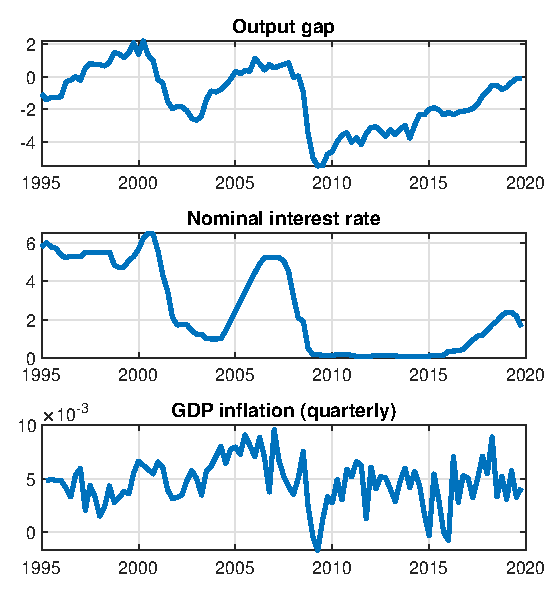
\includegraphics[width = 0.9\textwidth]{figures/dataplot.eps}
\end{columns}
\end{frame}


\begin{frame}{Linking model and data set}
\begin{wideitemize}
\item We extend the model with a set of \hi{observation equations} linking data and model variables.
\begin{itemize}
    \item Recall that all steady states are zero in our model (demeaned).
    \item One period corresponds to one quarter in the model.
    \item An amazing resource by Johannes Pfeifer: \href{https://drive.google.com/file/d/1r89OU5OE3CBa6tOlj6l3hNVWEaRH5Anv/view?usp=sharing}{A Guide to Specifying Observation Equations for the Estimation of DSGE Models}
\end{itemize}
\item Specify \hi{observed variables} after \texttt{varobs} command.
\item \hi{Declare dataset} via a \texttt{*.mat}-file or as an m-file
\begin{itemize}
    \item Example: \texttt{estimation(datafile=examplefile)}
\end{itemize}
\item Typically, the data feature a trend: Many options to deal with it!
\end{wideitemize}
\end{frame}

\begin{frame}[fragile]{Observation equations (cont'd)}
We need new variables and parameters (and calibrate the latter)
\begin{minted}{c++}
var
pieobs     ${\pi^{obs}}$ (long_name = 'Observed inflation')
ygapobs    ${y^{obs}}$   (long_name = 'Observed output gap')
inomobs    ${i^{obs}}$   (long_name = 'Observed nom. interest rate')
;

parameters
inomss   ${\bar{i}}$     (long_name = 'Mean interest rate')
piess    ${\bar{pi}}$    (long_name = 'Mean inflation')
;
\end{minted}
\end{frame}

\begin{frame}[fragile]{Observation equations (cont'd)}
\begin{minted}{c++}
model;

[name='Observation equation ygap']
ygapobs = y*100;

[name='Observation equation inflation (quarterly)']
pieobs = pie + piess;

[name='Observation equation interest rate']
inomobs = inom*400 + inomss;

end;
\end{minted}
\end{frame}




\begin{frame}{Why Bayesian?}
\begin{wideitemize}
\item Attractive underlying paradigm...
\item ...but for many macroeconomists its practicality
\item Avoids ``dilemma of absurd parameter estimates'' sometimes arising under pure maximum likelihood
\begin{itemize}
\item Structural parameter estimates at odds with outside evidence (e.g. from microfoundations).
\item Prior information can be brought it in: Macro time series sometimes not informative enough to discriminate among different theories
\end{itemize}
\item Model comparison is easy (even for non-nested models)
\item It's a system estimation method 
\end{wideitemize}
\end{frame}

\begin{frame}{Elements of Bayesian analysis}
\begin{wideitemize}
\item A Bayesian model consists of data $Y$ and parameters $\theta$ with a joint distribution $p(Y,\theta)$
\item \hi{Priors} contain information on parameters not included in the data: $p(\theta)$ (initial information independent of the data)
\item \hi{Likelihood} function based on the data: $L(Y,\theta)$
\begin{itemize}
    \item Likelihood of observing particular data $Y_{1:t}$ as a function of the parameters $\theta$.
    \item We are interested in finding $\theta$ that maximises the likelihood.
\end{itemize}
\item \hi{Posterior distribution} $p(\theta|Y)$ as a combination of prior and likelihood via Bayes theorem
\begin{itemize}
    \item This is a (potentially very complicated) probability distribution.
\end{itemize}
\end{wideitemize}
\end{frame}

\begin{frame}{Bayes theorem}
\begin{wideitemize}
\item Recall Bayes rule\footnote{Simply combine $p(A,B)=p(A|B)p(B)$ and $p(A,B)=p(B|A)p(A)$}
\begin{equation*}
     p(A|B) = \frac{p(B|A)p(A)}{p(B)}
\end{equation*}
\item In our case with $\theta$ as $A$ and the data $Y$ as $B$, we can define the \hi{posterior distribution} as 
\begin{equation*}
     p(\theta|Y) = \frac{L(Y,\theta)p(\theta)}{p(Y)} \propto L(Y,\theta)p(\theta)
\end{equation*}
\item $p(Y)$, the \hi{marginal data density}, is independent of the likelihood (probability of observing the data).
\begin{itemize}
    \item Can be used for model comparison.
\end{itemize}
\end{wideitemize}
\end{frame}

\begin{frame}{Specifying priors}
\begin{wideitemize}
\item Priors bring in \hi{information not included in the data}. They are random variables with probability distributions.
\item Can come from micro data, other papers, ...
\item Commonly used prior distributions:
\begin{itemize}
    \item \textit{Beta} distribution for parameters between 0 and 1 (e.g. shock persistence)
    \item \textit{Gamma} and \textit{Inverse Gamma} distributions for parameters restricted to be positive (e.g. shock standard deviation)
    \item \textit{Normal} distribution.
    \item \textit{Uniform} distribution.
\end{itemize}
\item Always check the plots to verify that your priors look sensible!
\item Simulate the model with the prior specification
\end{wideitemize}
\end{frame}

\begin{frame}[fragile]{Specifying priors: Example}
\begin{minted}{c++}
estimated_params;
rho_a,,,,BETA_PDF,0.8,0.1;
rho_c,,,,BETA_PDF,0.8,0.1;
rho_i,,,,BETA_PDF,0.5,0.1;
stderr u_a,INV_GAMMA_PDF,0.0025,2;
stderr u_c,INV_GAMMA_PDF,0.0025,2;
stderr u_i,INV_GAMMA_PDF,0.0025,2;
end;       
\end{minted}
\end{frame}

% \begin{frame}{Bayes theorem and the posterior}
% \begin{wideitemize}
% \item 
% \end{wideitemize}
% \end{frame}

\begin{frame}{Likelihood}
\begin{wideitemize}
\item For a given set of parameters $\theta$, we can solve the (linearised) model with Dynare and obtain a state space representation (more complex for OBCs):
\begin{equation*}
    X_t = T(\theta)X_{t-1} + C(\theta)u_t
\end{equation*}
\item Common problem: We rarely observe all variables in the data $Y_t$, formalised by the observation equation (here without measurement error)
\begin{equation*}
    Y_t = H(\theta)X_{t}
\end{equation*}
\item However, to evaluate the likelihood function, we need all model variables.
\item Key: Need to use a filter!
\end{wideitemize}
\end{frame}



\begin{frame}{Likelihood: Kalman filter}
\begin{wideitemize}
\item The Kalman filter is a very efficient recursive algorithm to construct the likelihood.
\item There must be at least as many shocks as observables to avoid stochastic singularity.
\item Full derivation in Hamilton's textbook.\footcite{hamilton2020time}
\item We will encounter the \hi{piecewise-linear Kalman filter} (PKF) later in more detail.
\end{wideitemize}
\end{frame}


   
\begin{frame}{Posterior}
\begin{wideitemize}
\item The posterior $p(\theta,Y)$ is a full distribution, typically not analytically tractable.
\item But we can easily get its value for a given parameter vector $\theta$
\item We can then use numerical methods to find the mode %(i.e. the value of $\theta$).
\item For further calculations, main problem: We cannot directly draw from the posterior distribution.
\item In general, however, we are interested in averages (expected values):
\begin{equation*}
    E\left[g(\theta|Y)\right] = \int g(\theta)p\left(\theta|Y\right)d\theta
\end{equation*}
\end{wideitemize}
\end{frame}

\begin{frame}{MCMC}
\begin{wideitemize}
\item Idea: Use \hi{Monte Carlo} integration by sampling $S$ draws from the posterior distribution
\begin{equation*}
    E\left[g(\theta|Y)\right] = \int g(\theta)p\left(\theta|Y\right)d\theta \approx \frac{1}{S}\sum_{s=1}^Sg(\theta_s)
\end{equation*}
\item Typically, we apply Markov Chain Monte Carlo Methods (MCMC), in particular the \hi{Metropolis-Hastings Algorithm}
\item The main idea: Efficiently explore the distribution! \texttt{mh\_jscale} allows you to target an acceptance rate (should be around 0.24).
\item MCMC generates (correlated) sequences \textit{as if} directly drawn from the $p(\theta,Y)$.
\item Need to check whether this is indeed the case using diagnostic tools. Dynare does this for you! See the manual.
\end{wideitemize}
\end{frame}


\begin{frame}{Posterior draws}
\begin{wideitemize}
\item Once we have obtained the posterior draws, we can do many interesting things!
\item We can calculate object reflecting parameter uncertainty:
\begin{itemize}
    \item IRFs (e.g. how much does inflation increase following a demand shocks?)
    \item Moments
    \item Welfare measures
    \item ...
\end{itemize}
\end{wideitemize}
\end{frame}
   


\begin{frame}{Estimation steps in a nutshell}
\begin{wideenumerate}
\item Specify a prior distribution.
    \item Evaluate the likelihood function using a Kalman filter
    \item Compute the posterior mode.
    \item Approximate the posterior distribution using Markov Chain Monte Carlo methods (MCMC)
    \item Based on the posterior distribution, compute objects of interest: moments, IRFs, parameter uncertainty,...
\end{wideenumerate}
For a textbook treatment: See Herbst and Schorheide\footcite{herbst2015bayesian}
\end{frame}


\begin{frame}[fragile]{Forecasts, filtered, and smoothed variables }
\begin{wideitemize}
\item Command \texttt{filtered} computes a forecast based on past information ($I_{t-1}$)
\begin{equation*}
    x_{t|t-1} = E\left[x_t|I_{t-1}\right]
\end{equation*}
\begin{itemize}
    \item Specify horizon using \texttt{filter\_step\_ahead = [4:8]}
\end{itemize}
\item Command \texttt{smoother} computes the posterior distribution of all endogenous variables and shocks using all available information up to period $T$
\begin{equation*}
    x_{t|T} = E\left[x_t|I_{T}\right]
\end{equation*}
\begin{itemize}
    \item Dynare also always produces smoothed shocks.  
\end{itemize}
\item Command \texttt{forecast} computes forecast of 10 periods.
\begin{minted}{c++}
estimation(filtered_vars,smoother,forecast=10)
\end{minted}
\end{wideitemize}
\end{frame}



\begin{frame}{Savings time load mode files and continuing a chain}
\begin{wideitemize}
\item Often, you can avoid re-doing some computations.
\item For example, you can use a previous mode file (automatically produced by Dynare).
\begin{itemize}
    \item Specify \texttt{mode\_file=filename\_mode}
    \item and skip re-computation: \texttt{mode\_compute=0}
\end{itemize}
\item Or continue a previous Markov chain using \texttt{load\_mh\_file}
\item Example: \texttt{estimation(mode\_file=filename\_mode, mode\_compute=0,
load\_mh\_file)}
\item You can run the chains in parallel: A significant speed up! \url{https://www.dynare.org/manual/the-configuration-file.html\#parallel-configuration}
\end{wideitemize}
\end{frame}

\begin{frame}[fragile]{Some checks before launching the estimation}
\begin{wideitemize}
\item Initialise the filter using the calibration
\begin{minted}{c++}
estimated_params_init(use_calibration);
end;
\end{minted}
\item Run a smoother based on calibration, e.g.
\begin{minted}{c++}
calib_smoother(datafile=mydatafile) 
y ygapobs inom inomobs pie pieobs;
\end{minted}
\item Triple check the units and frequency of your observed variables
\end{wideitemize}
\end{frame}




\begin{frame}[fragile]{Code for estimation}
\begin{minted}{c++}
estimation(
    //mh_replic=0, // Draws from the chain
    presample = 20,
    mh_nblocks=1,//number of chains
    use_univariate_filters_if_singularity_is_detected=0,
    datafile=dataobsnkm,
    nodisplay, 
    mh_jscale = 0.9,//tune the accept. ratio
    first_obs=2,
    graph_format=(eps,fig), 
    smoother);
\end{minted}
\end{frame}


% \begin{frame}{Shock decompositions}
% \begin{wideenumerate}
% \item TBD
% \end{wideenumerate}
% \end{frame}

%\section[OBC Estimations]{Model estimation with occasionally binding constraints}
%\input{chapters/estimation_OBC.tex}

%\begin{frame}{Before concluding: General remarks}
\begin{wideitemize}
\item Always good to start simple:
\begin{wideitemize}
    \item Simpler models before complex (larger) models
    \item Simulation before estimation.
    \item Linear estimation before nonlinear
    \item Piecewise-linear before fully nonlinear.
\end{wideitemize}
\item Make use of the many resources (including Dynare summer school and Dynare forum)
\item It pays off to invest time into software tools such as version control with Git
\item Any issues with the PKF (and beyond): \href{mailto:philipp.pfeiffer@ec.europa.eu}{philipp.pfeiffer@ec.europa.eu}
\end{wideitemize}
\end{frame}


\begin{frame}{Wrapping up}
\begin{wideitemize}
\item This course was a primer into easily accessible tools for macroeconomic analysis with occasionally binding constraints.
\item We have covered different simulation routines.
\item And touched upon econometric evaluations of DSGE models.
\item We have focused on \hi{scalable} methods.
\pause
\item I am around until the end of the week and happy to meet and discuss models with OBCs, research, economics, ... and learn about Lithuania and the Baltics.
\item \hi{\textbf{Thank you very much!}}
\end{wideitemize}
\end{frame}

%\section*{Appendix}
%\begin{frame}
\textbf{Annex}
\end{frame}

\begin{frame}{Other nonlinear filtering methods in macroeconomics}
\label{details_lit}
\begin{wideitemize}
\item Boehl (2021) proposes a promising and very fast piecewise-linear solution algorithm.
\item Farmer (2021) provides a fast nonlinear approximation of the likelihood in non-Gaussian state space
models. 
\item Aruoba et al. (2020) exploit the piecewise-linear nature of OBCs for high-order solution
and particle filtering. 
\item These methods are particularly suitable for low-dimensional state-spaces but are
difficult to scale to models with more state variables.
\item For Markov-switching models, Maih (2015) provides efficient perturbation methods.
\end{wideitemize}
\hyperlink{lit}{\beamerbutton{Back}}
\end{frame}


\begin{frame}{PKF: Initialization}
\label{details_pkf_init}
\begin{wideitemize}
    \item Given the initial state mean and variance $x_0$ and $\mathbf{P}_0$, we denote their `best' estimate at any time $t-1$ $x_{t-1|t-1}, \mathbf{P}_{t-1|t-1}.$	
    \item Notation for state-dependent matrices: 
    \begin{eqnarray*}
    \mathbf{T}_{t|t}&=& \mathbf{T}(x_{t-1},\varepsilon_{t}) \\
    \mathbf{C}_{t|t}&=& \mathbf{C}(x_{t-1},\varepsilon_{t}) \\
    \mathbf{R}_{t|t} &=& \mathbf{R}(x_{t-1},\varepsilon_{t}),
    \end{eqnarray*}
\item Initialize the guess of the updated state matrices for iteration $j=0$
\begin{eqnarray*}
\mathbf{T}^{j}_{t|t}&=&\mathbf{T}_{t|t-1} \\
\mathbf{R}^{j}_{t|t}&=&\mathbf{R}_{t|t-1} \\
\mathbf{C}^{j}_{t|t}&=&\mathbf{C}_{t|t-1}. 
\end{eqnarray*}
\item Superscript $j$ denotes the iteration to find the state matrices.
\end{wideitemize}
\hyperlink{pkf_init}{\beamerbutton{Back}}
\end{frame}

\begin{frame}{PKF: Standard prediction and update step}
	\label{details_pred_upd}
\begin{itemize}
\item Given the guessed matrices, perform a prediction step
\begin{align*}
x^{(j)}_{t|t-1}&=\mathbf{T}^{(j-1)}_{t|t}\cdot x_{t-1|t-1}+\mathbf{C}^{(j-1)}_{t|t} \\
\mathbf{P}^{(j)}_{t|t-1}&=\mathbf{T}^{(j-1)}_{t|t}\cdot \mathbf{P}_{t-1|t-1}\cdot \mathbf{T'}^{(j-1)}_{t|t} +\mathbf{R}^{(j-1)}_{t|t}\cdot \mathbf{Q}\cdot \mathbf{R'}^{(j-1)}_{t|t}\\
y^{(j)}_{t|t-1}&=\mathbf{H} x^{(j)}_{t|t-1}\\
\mathbf{F}^{(j)}_{t}&=\mathbf{H}\cdot \mathbf{P}^{(j)}_{t|t-1}\cdot \mathbf{H}'\\
v^{(j)}{t}&= z_t-y^{(j)}_{t|t-1} 
\end{align*}
\item and an update step
\begin{eqnarray*}\label{eq:update1}
\mathbf{K}^{(j)}_t  &=&  \mathbf{P}^{(j)}_{t|t-1}\cdot\mathbf{H}'\\
x^{(j)}_{t|t} &=& x^{(j)}_{t|t-1}+\mathbf{K}^{(j)}_t \left(\mathbf{F}^{(j)}_{t}\right)^{-1}v^{(j)}_t  \nonumber\\ 
\mathbf{P}^{(j)}_{t|t} &=& \mathbf{P}^{(j)}_{t|t-1}-\mathbf{K}^{(j)}_t\left(\mathbf{F}^{(j)}_{t}\right)^{-1} {\mathbf{K}^{(j)}}'_t. \nonumber
\end{eqnarray*}
\item Here, each iteration $j$ follows the standard Kalman recursion.
\end{itemize}
	\hyperlink{pkf_pred_upd}{\beamerbutton{Back}}
\end{frame}





\begin{frame}[allowframebreaks]{Literature}
\printbibliography
\end{frame}

\end{document} 